\glsresetall
 \graphicspath{{figures/analysing/}}
\chapter{Introduction}\label{ch:intro}

The directivity of a sound sources is an issue that has an impact on many situations of our daily life, e.g. at live music venues. Voluntary listeners, namely the audience, enjoy comparatively high sound pressure levels when gathering around the stage. Non-voluntary listeners, generally neighbours, tend to perceive the sound emitted by the stage as a disturbing noise. This problem might be minimized with directivity control of the sound sources. The high sound energy will then be emits towards the audience, and less towards the neighbours. 


There are several effects that make this difficult, because commonly used loudspeaker contraptions for low frequency playback tend to act like omnidirectional sound sources. First, the dampening of sound in the air has significantly less influence on sound towards the lower frequency of the human hearing range than it has towards the higher frequency. Secondly, because of the way most houses are built, low frequency sound penetrates through walls and windows much more than high frequency sound. All of these effects lead to neighbours being disturbed by \textit{the low frequency} from nearby live music venues.\\
The difference in the perception of the sound is visualised in \autoref{fig:Problem}.


\begin{figure}[htbp]
	\centering
	\includegraphics[width=1\textwidth]{change_later.png}
	\caption{Normalized \gls{spl} in colour, red is high \gls{spl} where blue is low \gls{spl}}
		\label{fig:Problem}
\end{figure}

%\autoref{fig:Problem} shows the total sound pressure level \gls{spl} in \gls{db} from \SI{20}{\hertz} to \SI{20}{\kilo\hertz} for the voluntary listeners and the non-voluntary listeners during a concert.
\autoref{fig:Problem} shows a qualitative drawing of a near-ideal sound pressure distribution in the vicinity of a stage during a concert. The high-\gls{spl}areas are highlighted by red color, and is the area where the voluntary listeners condense. This area is define as the \textbf{participants' area} The non-voluntary listeners are located in the area around the participants' area, that we define as \textbf{the neighbourhood}. 

While a \gls{spl} distribution as depicted in \autoref{fig:Problem} is easier to achieve the higher the frequency gets, towards low frequencies the \gls{spl}distribution might look more like depicted in autoref(fig:problem2).



The directivity control of mid- and high frequency has a known solution which has been applied for many years. In general, horns are used, which are designed for a particular radiation pattern. Due to the long wave length in the low/mid- and low frequency range, the horns that are required to direct those wavelengths are not feasible for practical applications due to their size and weight. Therefore other, more space saving solutions have been developed and implemented in the last decade. It is possible to achieve a cardiod emission pattern by arranging subwoofers in a particular manner. Two or three subwoofers are pointed towards the participants' area and one subwoofer is pointed the opposite way. The signal for the subwoofer pointing away from the audience is processed to manipulate the phase.


This project aims towards applying a principle that has been put into commercial use in the D\&B audiotechnik SL-series, where the low/mid frequency directivity is controlled by signal processing four speaker unit. Two units are arranged in the front of the line array module and the other two arranged on each of the sides of the line array module.



\section{preliminary problem statement}
The following questions are made with the intention of gathering the necessary knowledge, to be able to answer a later stated problem statement. The preliminary questions, which will be answered in the analysis, are:

\begin{itemize}
\item In which frequency area do the line source speaker behave omnidirectional?
\item Which known technique is used to do the speaker cardioid?
\item Can a simulation be made which support D\&B audiotechnik claim?
\end{itemize}




%%%
\part{Problem Analysis}\label{pt:analysis} \glsresetall
 \graphicspath{{figures/analysing/}}
	\chapter{Directional characteristics of a loudspeaker}\label{ch:directional}
		\section{Origin}
Because this project is about shaping the directional characteristics of loudspeakers arrangements towards a particular direction, it is important to thorougly investigate the directional characteristic of a single loudspeaker cabinet. This serves as a baseline for comparison and also is essential, because the investigated cabinet will be used to form the speaker array later on.\\
In general, loudspeakers tend to display different directional behaviour depending on the frequency emitted. At low frequencies they can be viewed as omnidirectional sound sources. At higher frequencies the main direction of sound emission is in line with the motion direction of the voice coil. \citep{crocker98}
Depending on the ratio of the emitted wavelength to the diameter of the speaker, a radiation pattern with side lobes can occur. An analytic approximation to the behaviour can be made  when looking at a vibrating piston in an infinite baffel. However, this only takes into account the front side of the speaker. It is difficult to incorporate the effects of an enclosure into this model.\\
There are possibilities to numerically model the sound field around a speaker in a cabinet. However in the context of this project, conducting a measurement seems to be the most favourable approach towards quantifying the sound emitted by loudspeaker in the cabinet at numerous frequencies.
The knowledge gained through the measurements can then be used in order to designate a feasible frequency range for the beamforming.
		\section{Conclusion}
Bla Bla Nuclear Missile Bla
	\chapter{Analytical descriptions}\label{ch:analytical}
		\section{Single source}\label{ch:single_speaker_source}
To gain understanding about the interaction of several sources emitting sound simultaneously it is essential to first investigate the behaviour of a single sound source. In the context of this project loudspeakers are investigated. The goal of this section is to find a way to represent the sound emission of loudspeakers within the frequencies boundaries of this project (\SIrange{60}{300}{\hertz}).
The representation must be suffiencently accurate yet relatively simple to calculate in order to be useful in the optimization process that is a later part of this project (see \autoref{ch:optimization}).

%This section aims to introduce and analyse the fundamental for a single source, by analyse the behaviour of a baffled circular plane piston source. The pressure around the piston source will be analysed analytically, to determine the radiation of a single speaker from \SI{60}{\hertz} and upwards and compare it with the measurement from \autoref{ch:polar_response}. The \SI{60}{\hertz} lower limit enable the simulation to be validated by measurement in the AAU anechoic chamber and is a used lower limit for the low/mid driver in some line source array \citep{V-DOSC}.  The analyse shall end out with a approximated simulation model of the \gls{dut}.
\subsection{Pressure emission from an omidirectional source}\label{ssec:omni}
As explained in \autoref{ch:polar_response} loudspeakers are commonly treated as omnidirectional sources at low frequencies. Taking advantage of this approximation, the sound pressure emission in free field conditions can be described conveniently. \citep[p. 171]{Kinsler2000} state the following equation \autoref{eq:omni_source} for a pulsating sphere. It has to be noted, that the position of the sphere in the given case is the acoustic center of the loudspeaker (see \autoref{sec:ac_center}).
\begin{equation}\label{eq:omni_source}
p(r,t)\,=\,\rho_0 c V_0 \left(\frac{a}{r}\right)\cos \theta_a \textbf{\textit{e}}^{j\left(\omega t - k(r-a)+\theta_a\right)}
\end{equation}
\startexplain
\explain{$p$ is the sound pressure.}{\si{\pascal}}
\explain{$r$ is the distance, for which the pressure is being calculated, \(r>a\).}{\si{\meter}}
\explain{$t$ is the time, for which the pressure is being calculated.}{\si{\meter}}
\explain{$\rho_0$ is the specific density of air.}{\si{\kilo\gram\per\cubic\meter}}
\explain{$c$ is the speed of sound.}{\si{\meter\per\second}}
\explain{$V_0$ ist the peak velocity at the surface of the spherical source.}{\si{\meter\per\second}}
\explain{$a$ is the radius of the spherical source.}{\si{\meter}}
\explain{$\theta_a$ is equal to $\tan(ka)$.}{\si{1}}
\explain{$\omega$ is the angular frequency.}{\si{\second^{-1}}}
\explain{$k$ is the wavenumber.}{\si{\meter^{-1}}}
\stopexplain

\subsection{Pressure emission from a baffled piston}\label{ssec:piston}
Another  approach to analytically approximate the behaviour of a cone loudspeaker is given by \citep[p. 179 ff.]{Kinsler2000}, where the behaviour of the sound radiated from a plane circular piston surrounded by an infinte rigid baffle is described. The piston model is derived from the model of a continous line source as described in \citep[p. 176 f.]{Kinsler2000}.


%To characterize the directional properties of an analytical model of the \gls{dut}, the source will be modulated in two dimension as one baffled circular plane piston source. The analysis of a piston source in two dimension built on a thin piston source in three dimension where the x axis is fixed in the plot. This is possible because of vertical beam patten symmetry of \autoref{fig:continues_line_source} \citep{Kinsler2000}. The piston lays flat down so i look like a line source and have radius $a$. The baffled circular plane piston source can be considered as many continuous line sources, which detonate dx and is pointing towards the reader on \autoref{fig:continues_line_source}. The calculated pressure point will be in far field where $r>>a$ holds and the surface integral can be rewritten to a Bessel function \citep{Kinsler2000}. The pressure formula is therefore:

\begin{equation}\label{eq:piston_source}
p(r,\theta ,t)=\frac{j}{2} \rho_{0}c  V_{0}\frac{a}{r}ka \left ( \frac{2J_1(ka\, sin(\theta ))}{ka\, sin(\theta )} \right )e^{j(\omega t-kr)}
\end{equation}
\startexplain
	\explain{$r$ is the distance, for which the pressure is being calculated, \(r>a\).}{\si{\meter}}
	\explain{$\theta$ is the angle at which the pressure is calculated, relative to the direction, in which the piston is moving.}{\si{1}}
	\explain{$t$ is the time, for which the pressure is being calculated.}{\si{\meter}}
	\explain{$j$ is the imaginary unit}{\si{1}}
	\explain{$\rho_0$ is the specific density of air.}{\si{\kilo\gram\per\cubic\meter}}
	\explain{$c$ is the speed of sound.}{\si{\meter\per\second}}
	\explain{$V_0$ ist the peak velocity of the piston.}{\si{\meter\per\second}}
	\explain{$a$ is the radius of the piston.}{\si{\meter}}
	\explain{$k$ is the wavenumber.}{\si{\meter^{-1}}}
	\explain{$J_1$ is the Bessel function of the first kind of order 1.}{\si{1}}
	\explain{$\omega$ is the angular frequency.}{\si{\second^{-1}}}
\stopexplain

A major disadvantage to utlizing the piston model in the context of the project is, that no information about the cabinet of the \gls{dut} is incorporated. The concept of an infinite rigid baffle leads to results that are axis symmetric along the \SIrange{-90}{90}{\degree}-line in a polar plot. This is illustrated in \autoref{fig:piston_analytical}.
\begin{figure}[H]
	\centering
	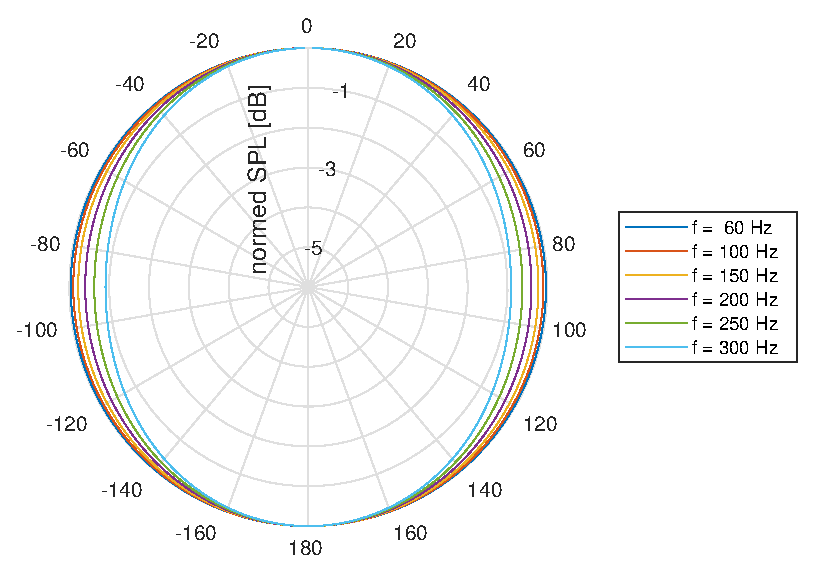
\includegraphics[width=0.7\textwidth]{piston.eps}
	\caption{normed SPL according to \autoref{eq:piston_source}, $a=165.3$\si{\milli\meter}$\,\approx 13$'', corresponding to the size of \citep{seas33}.}
		\label{fig:piston_analytical}
\end{figure}
\autoref{fig:piston_analytical} displays almost perfect omnidirectional behaviour for lower frequencies and lowering pressure towards $\pm$\SI{90}{\degree} for higher frequencies. The deviation from omnidirectionality has the same qualitative appearance as the measured pressure curves in \autoref{fig:03_02_pressure_main}, however they significantly differ in numbers.
\begin{figure}[htbp]
	\centering
	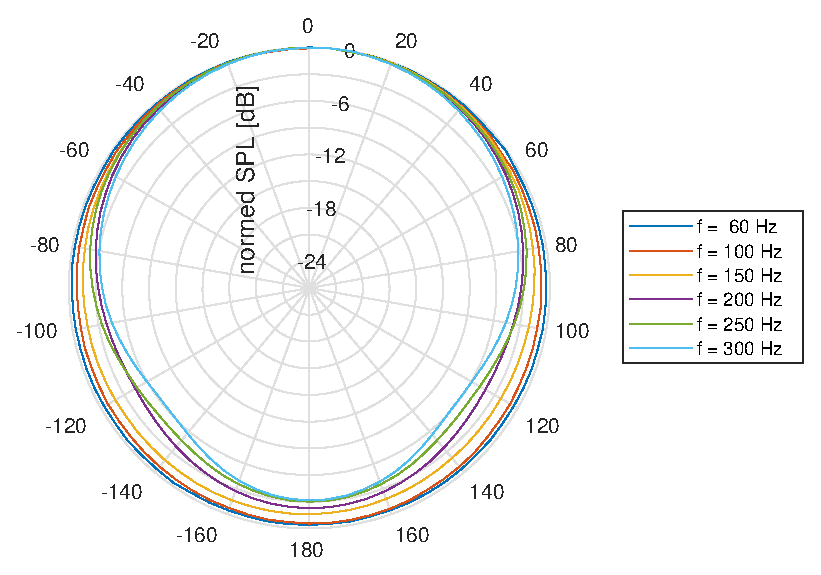
\includegraphics[width=0.7\textwidth]{03_02_meas1_pressure.eps}
	\caption{Normed \gls{spl}, measured at a distance \(d=\)\SI{2.74}{\meter}, see Appendix \ref{ax:directional_2}}
		\label{fig:03_02_pressure_main}
\end{figure}
\autoref{fig:03_02_pressure_main} also illustrates, that the solutions obtained with \autoref{eq:piston_source} do not realistically represent how the pressure is emitted on the back side of the speaker. Specifically, the indents in the in the curves for frequencies $\ge$\SI{200}{\hertz} at approx. $\pm$\SI{125}{\hertz} in \autoref{fig:03_02_pressure_main} deviate from the shape that is drawn by the piston model.
%The movement of the surface is described with

%\begin{equation}
%v = V_{0} \cdot exp(j \omega t)
%\end{equation}

%\startexplain
%    	\explain{$v$ is the complex speed of the line source }{\si{1}}
%        \explain{$V_{0}$ is the Amplitude}{\si{1}}
%        \explain{$j$ is the imaginary unit }{\si{1}}
%        \explain{$\omega$ is the angular velocity }{\si{1}}
%        \explain{$t$ is the time }{\si{1}}
%\stopexplain
    
%Each small sources is treated as an baffled simple source with a width of $dx$ and the source strange can be modulated as following      
%
%\begin{equation}
%dQ = V_{0} 2 a\, sin(\phi) \, dx
%\end{equation}
%
%    \startexplain
%    		\explain{$dQ$ is the simple source strange }{\si{1}}
%        \explain{$V_{0}$ is the Amplitude}{\si{1}}
%        \explain{$a$ is the radius for cylinder }{\si{1}}
%        \explain{$\phi$ is the angle between the radius $a$ and the x axis}{\si{1}}
%        \explain{$dx$ is the length for the simple source }{\si{1}}
%    \stopexplain    
% 
%The following \autoref{fig:continues_line_source} shows an example of the continues line source where one of the small source is showed with width $dx$ and length $2a \, sin(\phi)$. 
%
%\begin{figure}[H]
%	\centering
%\begin{picture}(0,0)%
%\includegraphics{line_source.pdf}%
%\end{picture}%
%\setlength{\unitlength}{746sp}%
%%
%\begingroup\makeatletter\ifx\SetFigFont\undefined%
%\gdef\SetFigFont#1#2#3#4#5{%
%  \reset@font\fontsize{#1}{#2pt}%
%  \fontfamily{#3}\fontseries{#4}\fontshape{#5}%
%  \selectfont}%
%\fi\endgroup%
%\begin{picture}(31223,16833)(-5411,-436)
%\put(12106,7139){r'}%
%\put(24121,15599){P(r,$\theta$,t)}%
%\put(946,2684){$\theta$}%
%\put(23851,659){x}%
%\put(-89,16094){z}%
%\put(11341,8354){r}%
%\put(3466,-571){$a$}%
%\put(1441,-376){$dx$}%
%\put(-134,-421){0}%
%\put(-4049,-571){$-a$}%
%\put(226,1649){$\Delta$r}%
%\end{picture}%
%	\caption{The model of a continues line source where y axis is pointing towards the reader. (ref the book)}
%		\label{fig:continues_line_source}
%\end{figure}




%\subsection{Comparison: calculations based on the baffled piston and measured polar respone}
%In this section, the \gls{dut} will be simulated as a baffled circular plane piston source as described in \autoref{ch:single_speaker_source} and compared to the actually measurement of the \gls{dut} \autoref{ax:directional_2}. An piston simulated model of \citep{seas33} in MATLAB shows in \autoref{fig:piston_model_of_seas33}
%
%\begin{figure}[H]
%	\centering
%	\includegraphics[width=0.8\textwidth]{piston_model.pdf}
%	\caption{The figure shows  The \gls{dut} which correspond to this figure is a \citep{seas33}}
%		\label{fig:piston_model_of_seas33}
%\end{figure}
%
%The actually measurement of the \citep{seas33}  \autoref{ax:directional_2}.
%
%\begin{figure}[H]
%	\centering
%	\includegraphics[width=0.8\textwidth]{meas1_seas.pdf}
%	\caption{The figure shows  The \gls{dut} which correspond to this figure is a \citep{seas33}}
%		\label{fig:speaker_model}
%\end{figure}

\subsection{Fitting the omnidirectional source model to the \gls{dut}}\label{sec:correction}
The analytical descriptions of both the pulsating sphere (see \autoref{ssec:omni}) and the piston (see \autoref{ssec:piston}) do not describe the measured behaviour of the \gls{dut} in an adequate manner. In order to be able to perfom an optimization of the signal processing parameters for the speaker array (see \autoref{ch:optimization}), a sufficient model has to be obtained. For the sake of this project, it has been chosen to rely on measured data.
As the pressure and phase characteristic of the \gls{dut} have been ascertained in measurements (see Appendices \ref{ax:directional_1},\ref{ax:directional_2}), the measurements results can be processed to obtain a correction table relating to the model of the omnidirectional source. This is achieved by calculating a difference of the measured data from the ideal values, that would suggest omnidirectionality at any given frequency. The resolution of the correction grid is determined by angular resolution and the frequency resolution of the polar response measurement, that it is based on.  \autoref{fig:correction_3d} shows a pressure correction grid, based on the polar response from Appendix \ref{ax:directional_2}.
\begin{figure}[H]
	\centering
	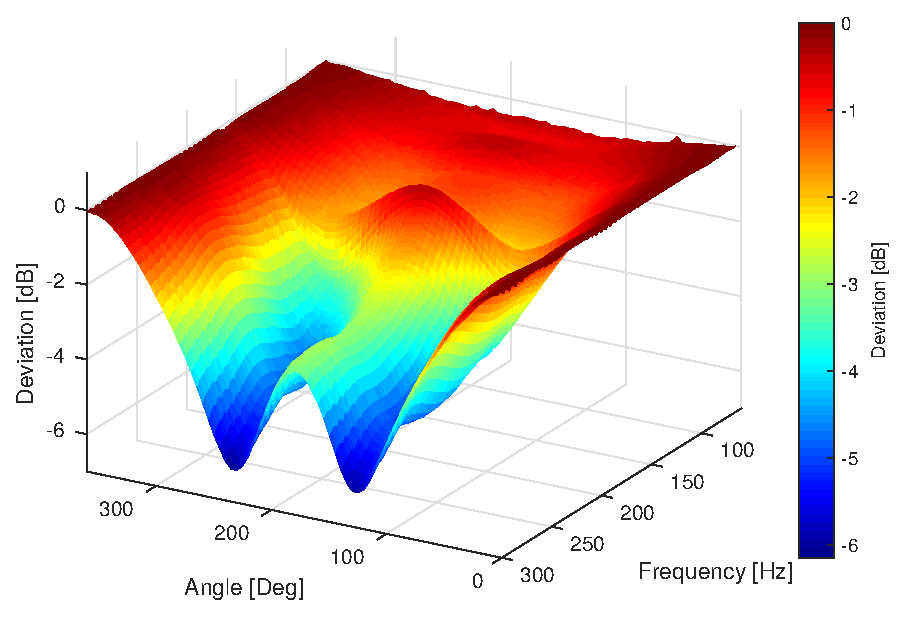
\includegraphics[width=0.7\textwidth]{correction_3d.eps}
	\caption{Contour plot of the pressure correction data, based on measurement data from Appendix \ref{ax:directional_2}}
		\label{fig:correction_3d}
\end{figure}
With the correction values applied, an augmented form of \autoref{eq:omni_source} can be established. Note, that while the deviation from omnidirectionality is visualized in \autoref{fig:correction_3d} in a \si{\decibel}-scale, for the usage in the \textsf{Dev}-function in \autoref{eq:aug_omni}, data has to be presented linearly.
\begin{equation}\label{eq:aug_omni}
p(r,t)\,=\,\rho_0 c V_0 \left(\frac{a}{r}\right)\cos \theta_a \textbf{\textit{e}}^{j\left(\omega t - k(r-a)+\theta_a\right)}\cdot\textsf{Dev}(f,\phi)
\end{equation}
\startexplain
\explain{$p$ is the sound pressure.}{\si{\pascal}}
\explain{$r$ is the distance, for which the pressure is being calculated, \(r>a\).}{\si{\meter}}
\explain{$t$ is the time, for which the pressure is being calculated.}{\si{\meter}}
\explain{$\rho_0$ is the specific density of air.}{\si{\kilo\gram\per\cubic\meter}}
\explain{$c$ is the speed of sound.}{\si{\meter\per\second}}
\explain{$V_0$ ist the peak velocity at the surface of the spherical source.}{\si{\meter\per\second}}
\explain{$a$ is the radius of the spherical source.}{\si{\meter}}
\explain{$\theta_a$ is equal to $\tan(ka)$.}{\si{1}}
\explain{$\omega$ is the angular frequency.}{\si{\second^{-1}}}
\explain{$k$ is the wavenumber.}{\si{\meter^{-1}}}
\explain{$\textsf{Dev}$ is the pressure deviation from the correction table.}{\si{1}}
\explain{$f$ is the frequency.}{\si{\hertz}}
\explain{$\phi$ is the angle, for which the pressure is being calculated relative to the main axis of the speaker.}{\si{1}}
\stopexplain
\section{Conclusion of single source}
Investigating analytical ways to express the behaviour of a speaker by incorporation no other information then its size leads to results that are not particulary accurate and are therefore of limited use. While it appears to be possible to get better estimates by incorporating more information into a numerical model (e.g. \citep{vanderkooy10}). The given objective of using the model for an optimization makes this approach unfeasible. Because measurements have been conducte investigating the directional characteristics of the loudspeaker that will later be used, a more empirical approach has been found. Exploiting information from the measurements, the relatively simple model of a pulsating sphere can be augmented, so that it fits the behaviour of the \gls{dut}.
		\input{chapters/analysing/zero_order_gradient}
		\input{chapters/analysing/first_order_gradient}
		\input{chapters/analysing/dimension_limit}

	



%%
\part{Design and Optimization}\label{pt:design} 
\graphicspath{{figures/design/}}
	\chapter{Hardware Configuration}
		%\input{chapters/design/dspchoice}
	\chapter{Determining SP-Parameters}\label{ch:optimization}
		\section{Problem Description}
In order to realize a directional low-mid emission with the chosen speaker configuration, signal parameters have to be chosen in a specific manner. The directional characteristics of the speaker array depend on the amplitude and phase of the signal that is transduced via the individual speakers. The resulting directional characteristics of a given set of signal-parameters can be described by the use of a analytical model, that has been supplemented with knowledge from measuring the polar response of the speakers.\\
Assuming, that the model describing the directional characteristics of the array, is sufficiently accurate, it is possible to form an optimization problem. Any set of \gls{sp} parameters can be evaluated by plugging it into the supplemented analytical model. Solutions, that resemble the desired directional characteristic are considered optimal.\\
The supplemented analytical model describes intricate physical behaviour and is related to the desired behaviour of the speaker array.  This makes it favourable to approach the given problem with combinatorial optimization. Specifically, it has been chosen to handle the problem with a \gls{ga}, where the supplemented analytical model used to evaluate the \textit{fitness}.


\section{\gls{ga}: Fundamentals} 		
	\chapter{Filter Development}
	\section{Filter}\label{sec:filter_design}

The aim of this chapter is to analyse the data from \ref{sec:opt_result} and choose the implementation method. From the beam forming optimization \autoref{sec:genetic_con} it was concluded that there shall be a cost filter and a beam forming filter. This chapter starts analyse the cost filter and design a filter solution, then the beam forming filter will be analysed and a solution will be designed.


\section{The cost filter}
The analysis of the cost filter will be done only with respect to the gain of the transfer function and without taking the phase intro account. The reason to avoid the phase is that the filter is an input filter to the entire system, and therefore the phase of the filter will affect all speaker the same way and therefore not effect the beam forming. \\
To analyse the cost filter, the filter type and the slope or Q of the filter have to be determined. 

the filter type will be determined first. To determined the filter type, a second order polynomia estimation will be done on the data point of the cost filter. The polynomia estimation is done with MATLAB command \texttt{polyfit()} with a second order regression. This give a second order polinomia where  \texttt{polyval()} is used to estimate the filter transfer function. The estimation will be done from \SI{60}{\hertz} to \SI{400}{\hertz}. The \SI{400}{\hertz} choice is made such that the estimation fit at lest to the double frequency of beam forming interest. The following \autoref{} shows the estimate compare to the original data point.

\begin{figure}[H]
	\centering
	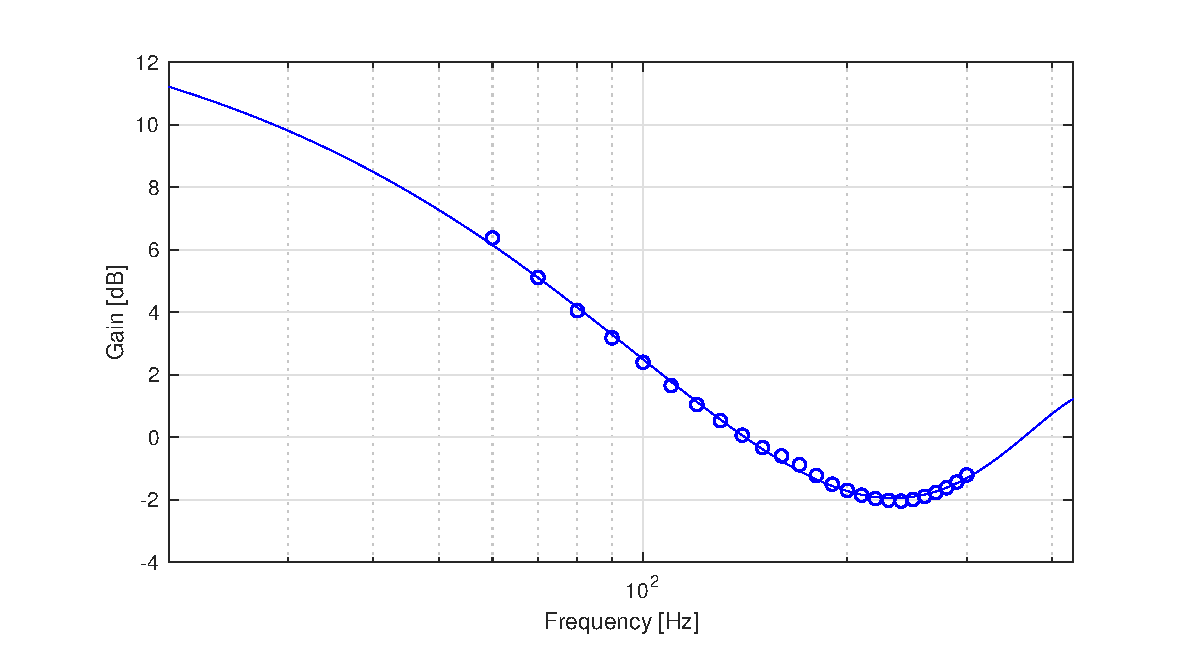
\includegraphics[width=1\textwidth]{band_stop_filter.eps}
	\caption{The graph shows transfer function of the estimated transfer function, where the blue  Solid line is the gain. All circle in the graph is the actual optimized point.}
		\label{fig:band_stop_filter}
\end{figure}


As it can be seen on \autoref{band_stop_filter} the shape of the estimated cost filter is a band stop filter with a relative gain of \SI{8.5}{\decibel}, and have a center frequency of \SI{175}{\hertz}. There needs to be a gain factor before the filter, to achieve the wanted band stop filter. The gain in the front of the filter will need to be \SI{6.4}{\decibel}. \\

\subsection{Parametric equalizer as cost filter}

Designing a bandstop filter is done with designing it as a bandpass filter, and use it in a feedback circuit. The following block diagram \autoref{} shows a block diagram a bandstop filter. 



To design a bandpass filter, the filter parameter is   



That means that the filter will be change to following \autoref{fig:band_pass_filter}


\begin{figure}[H]
	\centering
	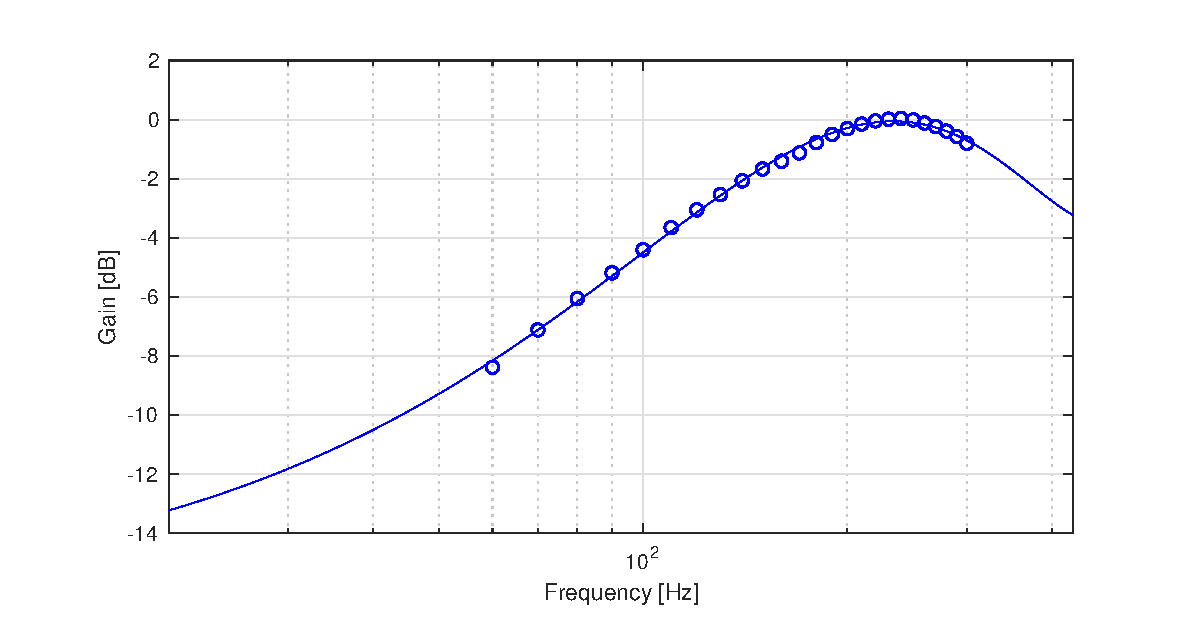
\includegraphics[width=1\textwidth]{band_pass_filter.eps}
	\caption{The graph shows transfer function of the estimated transfer function, where the blue  Solid line is the gain. All circle in the graph is the actual optimized point.}
		\label{fig:band_pass_filter}
\end{figure}

It can be seen on the figure, that the \SI{-3}{\decibel} bandwidth is \SI{213}{\hertz}, a center frequency of \SI{234}{\hertz} the gain must be \SI{8.5}{\decibel} 


\begin{figure}[H]
	\centering
	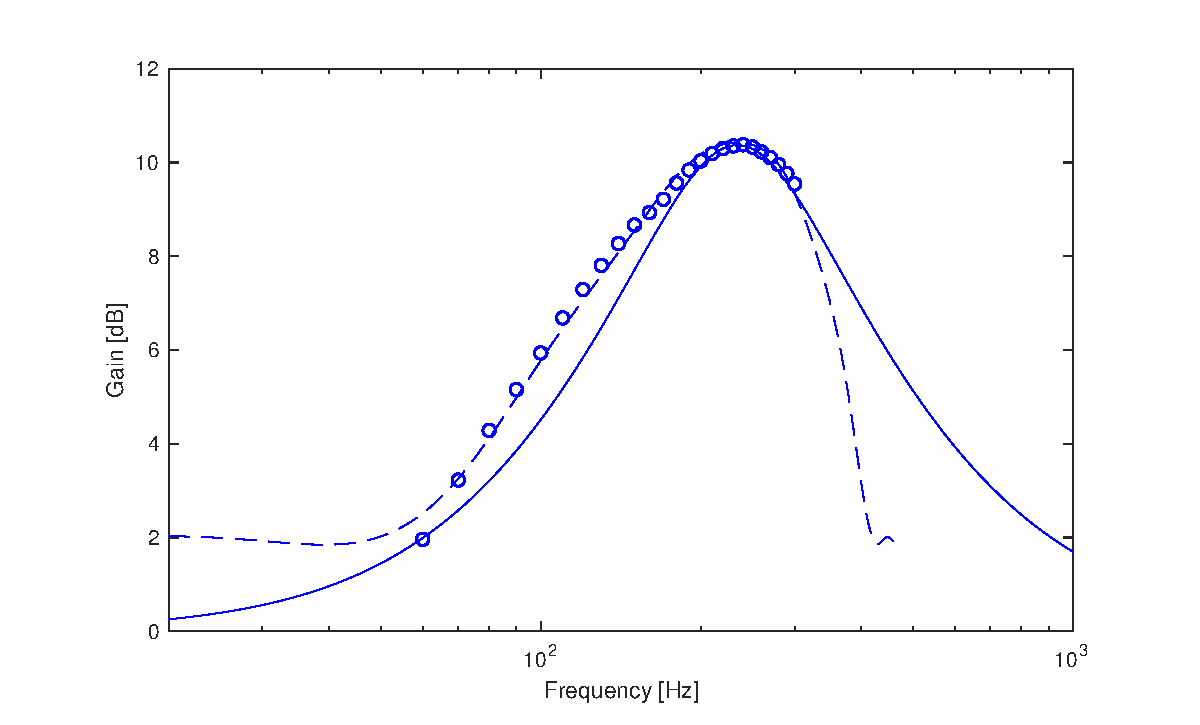
\includegraphics[width=1\textwidth]{band_pass_filter_h_non_scaled.eps}
	\caption{The graph shows transfer function of the estimated transfer function, where the blue  Solid line is the gain. All circle in the graph is the actual optimized point.}
		\label{fig:band_pass_filter_h_non_scaled}
\end{figure}

The wanted filter is raised by \SI{2}{\decibel} such that the designed filter also fit at low frequency. The output of the filter shall afterwards by atunuated by  \SI{2}{\decibel} to work as wanted.


It can be seen on \autoref{fig:band_pass_filter_h_non_scaled} that the \SI{-3}{\decibel} bandwidth is to narrov because the wanted filter have symmetrical shape in linear domain and not in logorithmic doman which the filter have.Therefore the filter bandwidth have to be extended with a factor of 1.1878. The factor is founded by trail and error. After the bandwidth is extended the filter is as following \autoref{fig:band_pass_filter_h}


\begin{figure}[H]
	\centering
	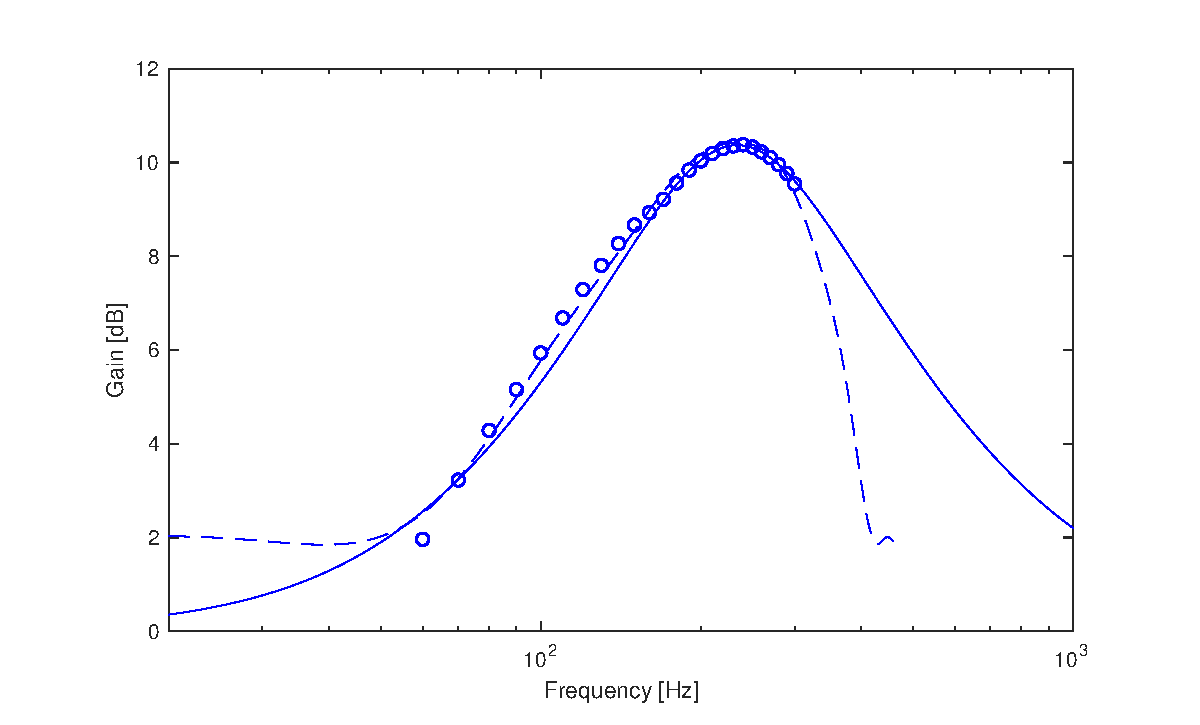
\includegraphics[width=1\textwidth]{band_pass_filter_h.eps}
	\caption{The graph shows transfer function of the estimated transfer function, where the blue  Solid line is the gain. All circle in the graph is the actual optimized point.}
		\label{fig:band_pass_filter_h}
\end{figure}


\subsection{Band stop filter form second order filter}
To transform a band pass filter to a band stop filter which not is a notch filter, the filter have to be transformed from a feed forward filter to a feedback filter 


(BLOCK DIAGRAM)

To transform the bandpass filter to a bandstop filter as descriped above, only the denominator and the numerator have to be switch around.

(The new formula)


\begin{figure}[H]
	\centering
	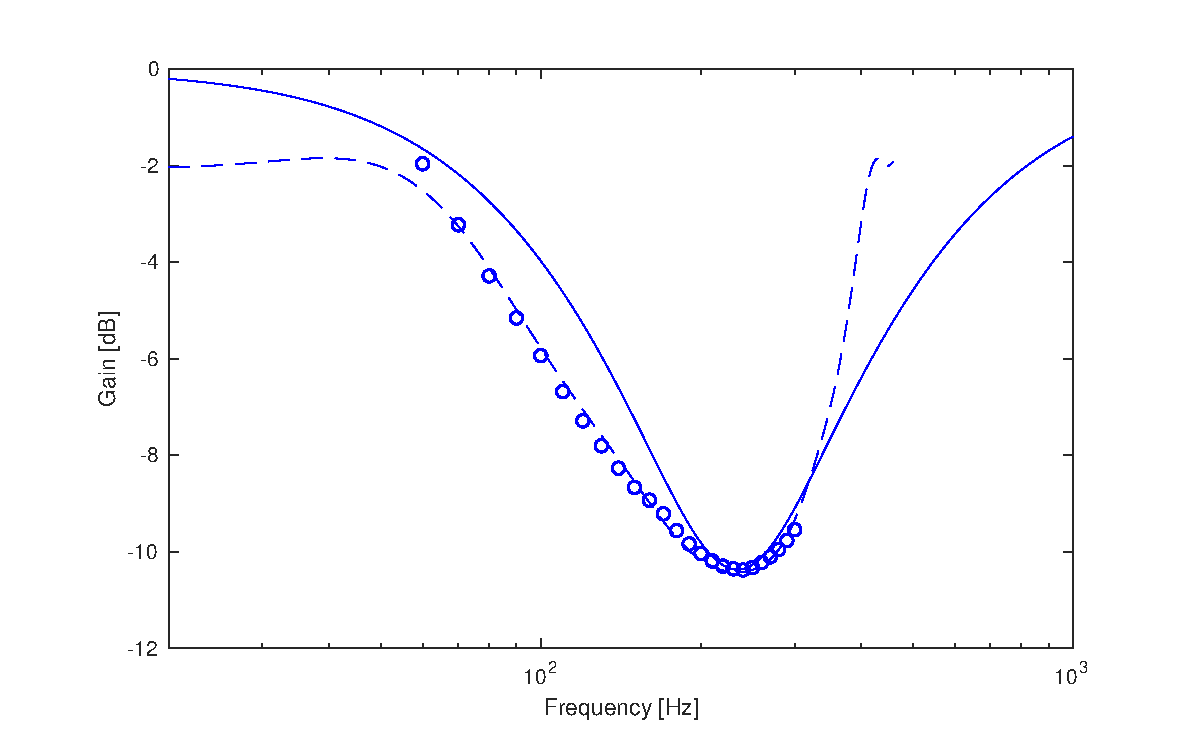
\includegraphics[width=1\textwidth]{band_stop_filter_non_scaled.eps}
	\caption{The graph shows transfer function of the estimated transfer function, where the blue  Solid line is the gain. All circle in the graph is the actual optimized point.}
		\label{fig:band_stop_filter_non_scaled}
\end{figure}


\begin{figure}[H]
	\centering
	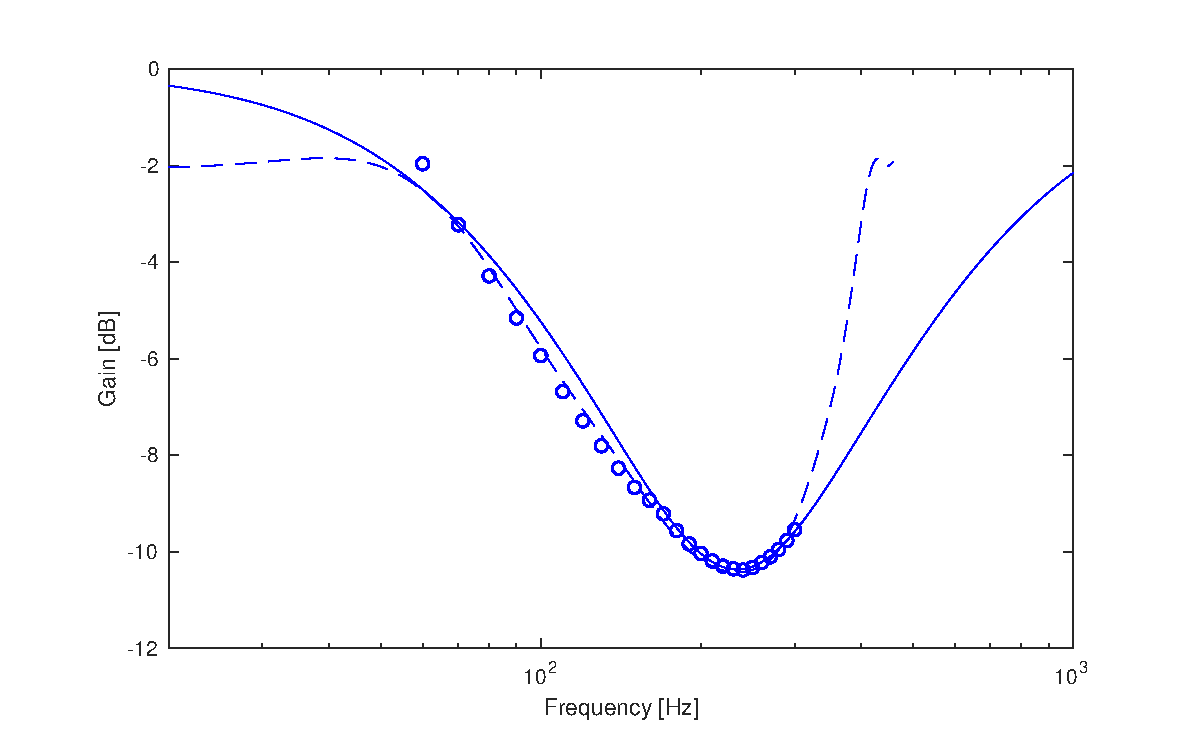
\includegraphics[width=1\textwidth]{band_stop_filter_scaled.eps}
	\caption{The graph shows transfer function of the estimated transfer function, where the blue  Solid line is the gain. All circle in the graph is the actual optimized point.}
		\label{fig:band_stop_filter_scaled}
\end{figure}


 The second step is to find the slope of the needed low pass filter. The slope is founded as following \autoref{eq:filter_slope}

\begin{equation}
\text{slope} = \frac{G_2\si{\decibel}-G_1\si{\decibel}}{\log_{10}{(f_2)}-\log_{10}{(f_1)}}
\end{equation}

    \startexplain
    \explain{$f$ is a frequency point }{\si{\hertz}}
    		\explain{$f_2$ is a frequency point higher that $f_1$ }{\si{\meter}}
        \explain{$G_1\si{\decibel}$ is the corresponding amplitude to $f_1$}{\si{\decibel}}
         \explain{$G_2\si{\decibel}$ is the corresponding amplitude to $f_2$}{\si{\decibel}}
    \stopexplain
    
The calculated slope is $17 \frac{\si{\decibel}}{dec}$ and it have been chosen that a standard first order low pass filter will be used. The following \autoref{} shows the error between the data and the filter. The error will make a pressure deference, that defence on frequency. 


\section{Beam forming filter}
The beam forming filter is not as easy as the cost filter to design, since that the phase and the gain have to be exact before the beam forming works. Therefore the phase have to be studied to determined the filter type. On the data point from the \ref{sec:opt_result} it can be seen that the phase is mostly linear in the frequency of interest, and therefore the filter will be a linear phase \gls{fir} filter. The smart thing with choosing a \gls{fir} filter is that the impulse response of the filter just have to be symmetric to achieve linear phase response. This means that optimizing the part of the impulse response and put it together with a mirrored version will always achieve linear phase. One disadvantages is that the cut off frequency is in the low frequency and therefore the filter order have to be high. \\

 A modified version of the genetic optimization algorithm will be used to find a optimized impulse response of the filter. To optimize the impulse respond of the filter, an estimate of the impulse respond have to be determined. One and the used way to estimate the impulse response is to transfer all polar coordinate to a complex rectangular transfer function and take the real of the \gls{ifft} of the complex transfer function. The polar to rectangular transform is done as following \autoref{eq:pol_to_regt}

\begin{equation}\label{eq:pol_to_regt}
x=rcos(\phi)+j \cdot rsin(\phi)
\end{equation}


     \startexplain
    \explain{$\phi$ is the angle of the transfer function in radian }{\si{1}}
        \explain{$r$ is the amplitude of the transfer function}{\si{1}}
        \explain{$j$ is the imaginary unit}{\si{1}}
    \stopexplain

The real of the \gls{ifft} gives an estimated impulse response but with a scaled cross over point. The meaning with scaled cross over point is that the cross over point follows the scaling of the sample frequency. With a sample rate of \SI{44.1}{\kilo\hertz} the following  \autoref{} shows the transfer function of the estimated impulse response. 

\begin{figure}[H]
	\centering
	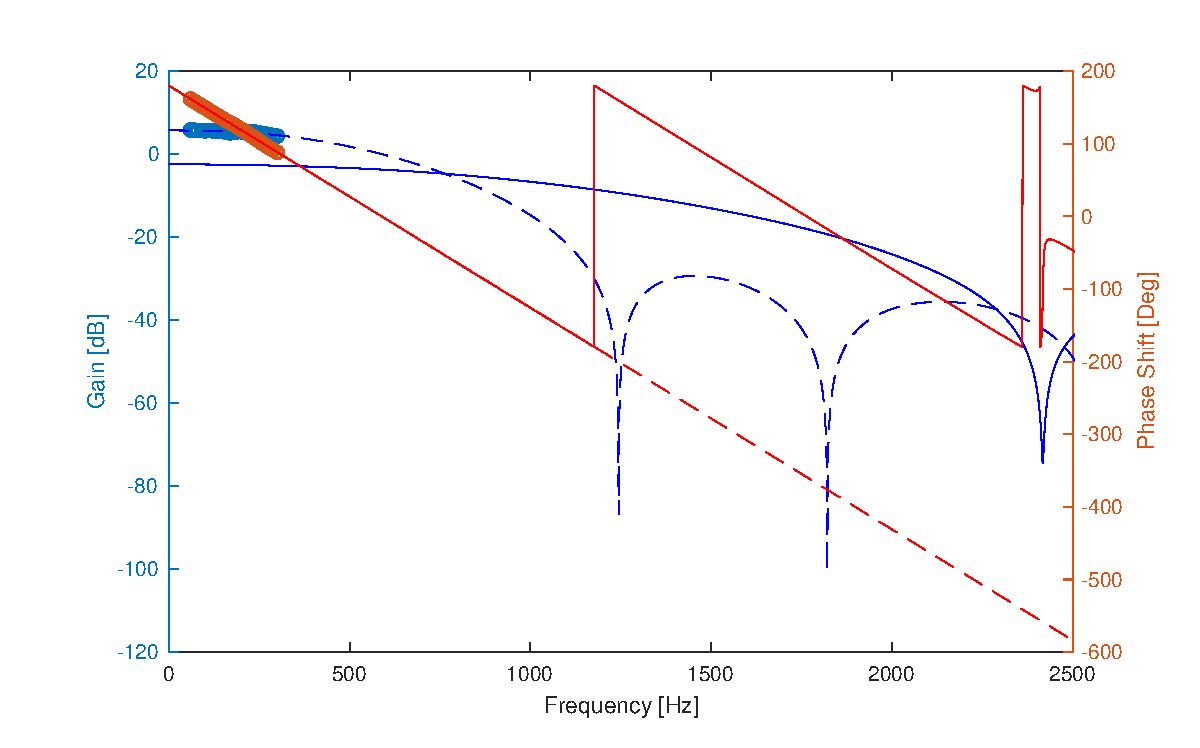
\includegraphics[width=1\textwidth]{ir_estimate_non_scaled.eps}
	\caption{The graph shows transfer function of the estimated impulse respond. The dashed line is transfer function that is needed for beam forming filter, where the blue line is the gain and the red line is the phase. The Solid line line is the transfer function of the estimated impulse response, where the blue line is the gain and the red line is the phase. All circle in the start of the graph is the actual optimized point.}
		\label{fig:ir_estimate_non_scaled}
\end{figure}


It can be seen that the cross over lays at a too high frequency and the gain at the frequency of interest is to low. The corresponding impulse response of the transfer function in \autoref{fig:ir_estimate_non_scaled} is as following \autoref{fig:ir_estimate_non_mirror} where the mirrored version not is added yet. 

\begin{figure}[H]
	\centering
	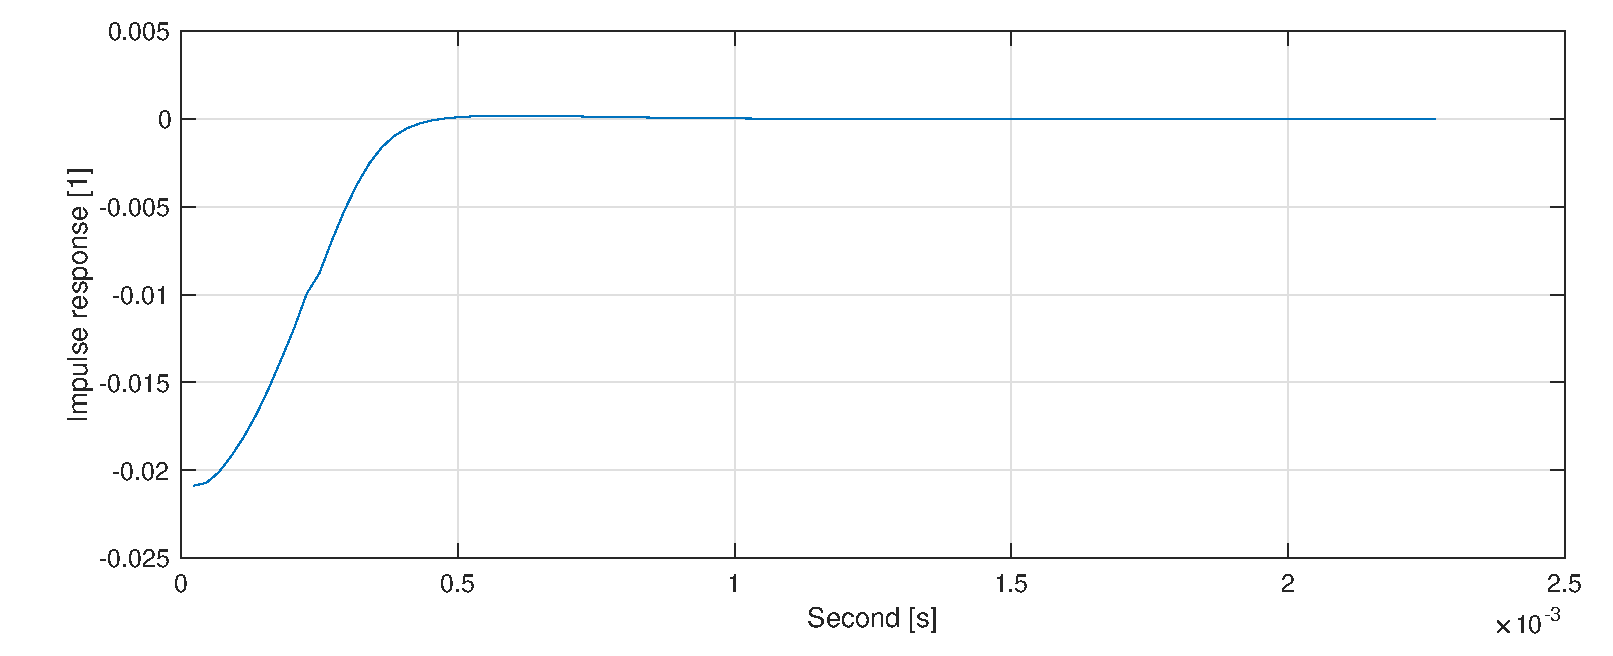
\includegraphics[width=1\textwidth]{ir_estimate_non_mirror.eps}
	\caption{The graph shows the impulse respond where the mirrored version is added to the impulse respond}
		\label{fig:ir_estimate_non_mirror}
\end{figure}

The version where the mirrored impulse response is added to the impulse response and the phase is matched to the wanted phase and is the corresponding impulse response to \autoref{fig:ir_estimate_non_scaled} is \autoref{fig:ir_estimate_mirror}

\begin{figure}[H]
	\centering
	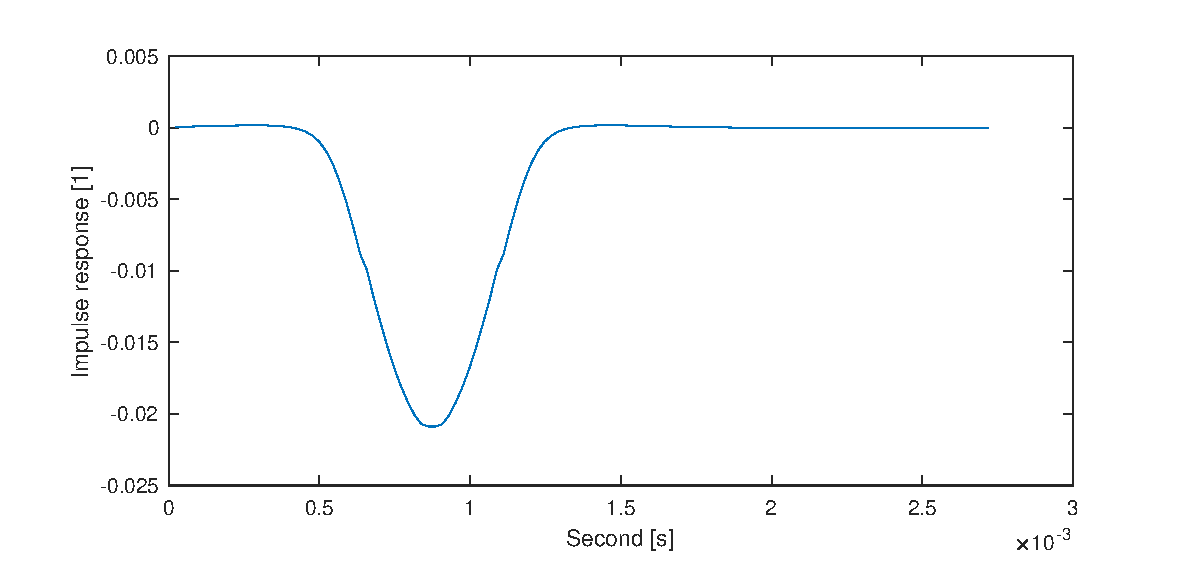
\includegraphics[width=1\textwidth]{ir_estimate_mirror.eps}
	\caption{The graph shows the impulse respond where the mirrored version is added to the impulse respond}
		\label{fig:ir_estimate_mirror}
\end{figure}


The impulse response have to be change the right way to make a good estimate. The way to lower the cross over point is to extend the part of the impulse respond that it have the highest amplitude, which also make the impulse response longer. Thinking about the theory of the \gls{fir} filter, that the lower cross over, the higher order the filter have to be and therefore the impulse respond gets longer. The following \autoref{} shows the estimated impulse respond that will be used for the optimization, where the crossover is approximatly where it shall be. 


\begin{figure}[H]
	\centering
	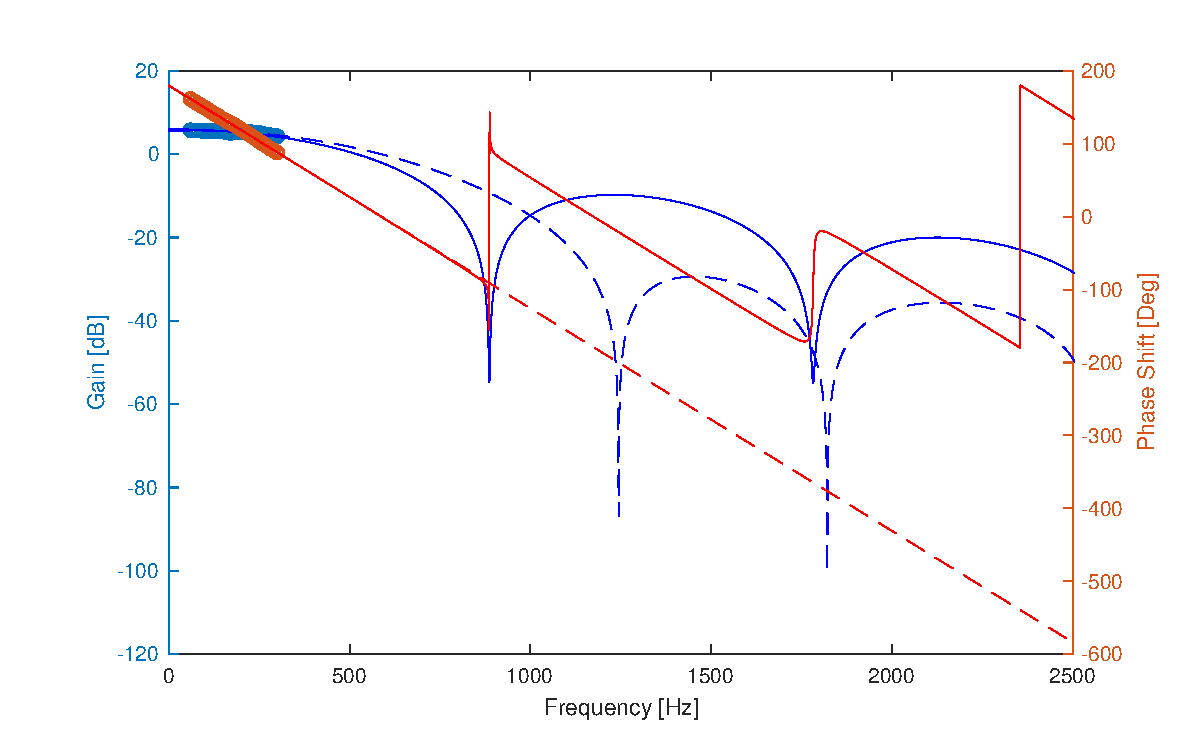
\includegraphics[width=1\textwidth]{ir_estimate_scaled.eps}
	\caption{The graph shows transfer function of the estimated impulse respond. The dashed line is transfer function that is needed for beam forming filter, where the blue line is the gain and the red line is the phase. The Solid line line is the transfer function of the estimated impulse response, where the blue line is the gain and the red line is the phase. All circle in the start of the graph is the actual optimized point.}
		\label{fig:ir_estimate_scaled}
\end{figure}


\begin{figure}[H]
	\centering
	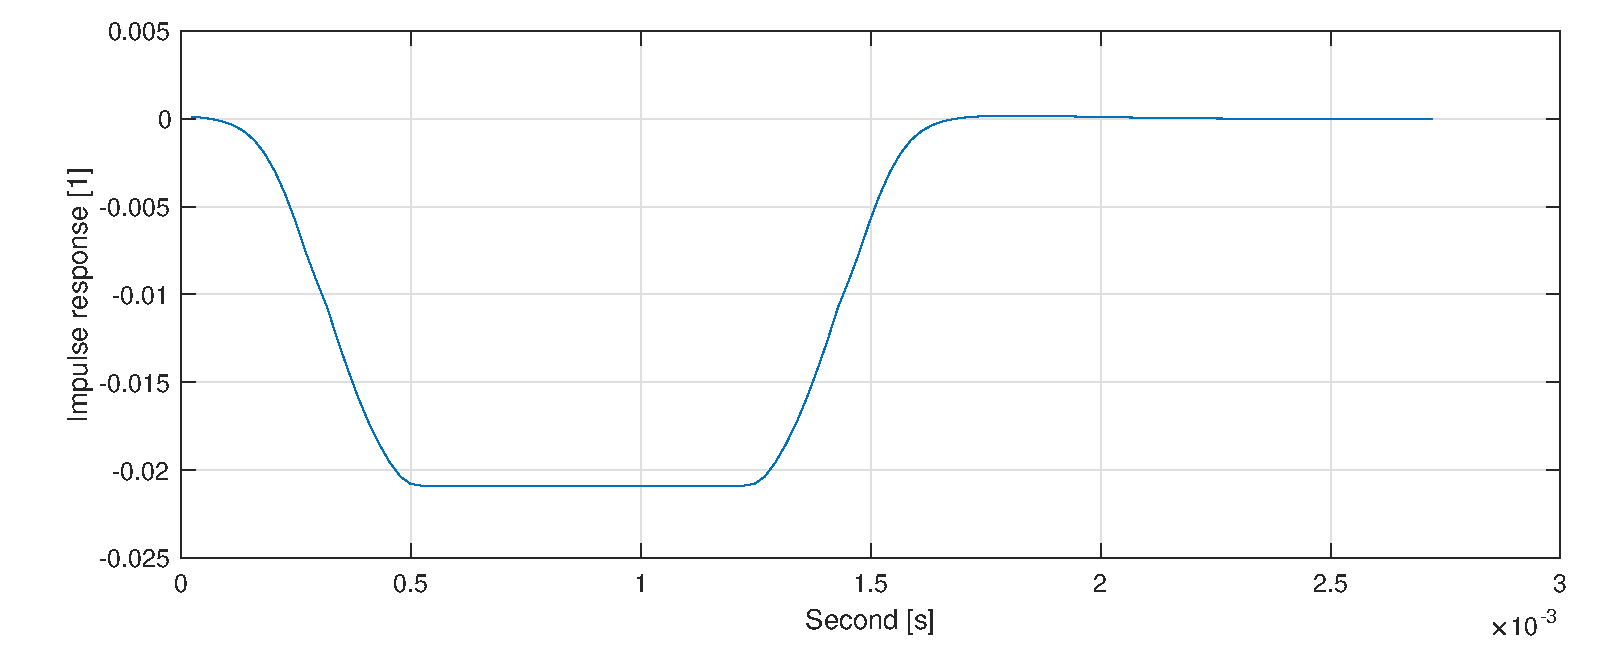
\includegraphics[width=1\textwidth]{ir_estimate_mirror_scale.eps}
	\caption{The graph shows the impulse respond where the mirrored version is added to the impulse respond}
		\label{fig:ir_estimate_mirror_scale}
\end{figure}

Where the corresponding impulse response is as \autoref{fig:ir_estimate_mirror_scale}

\begin{figure}[H]
	\centering
	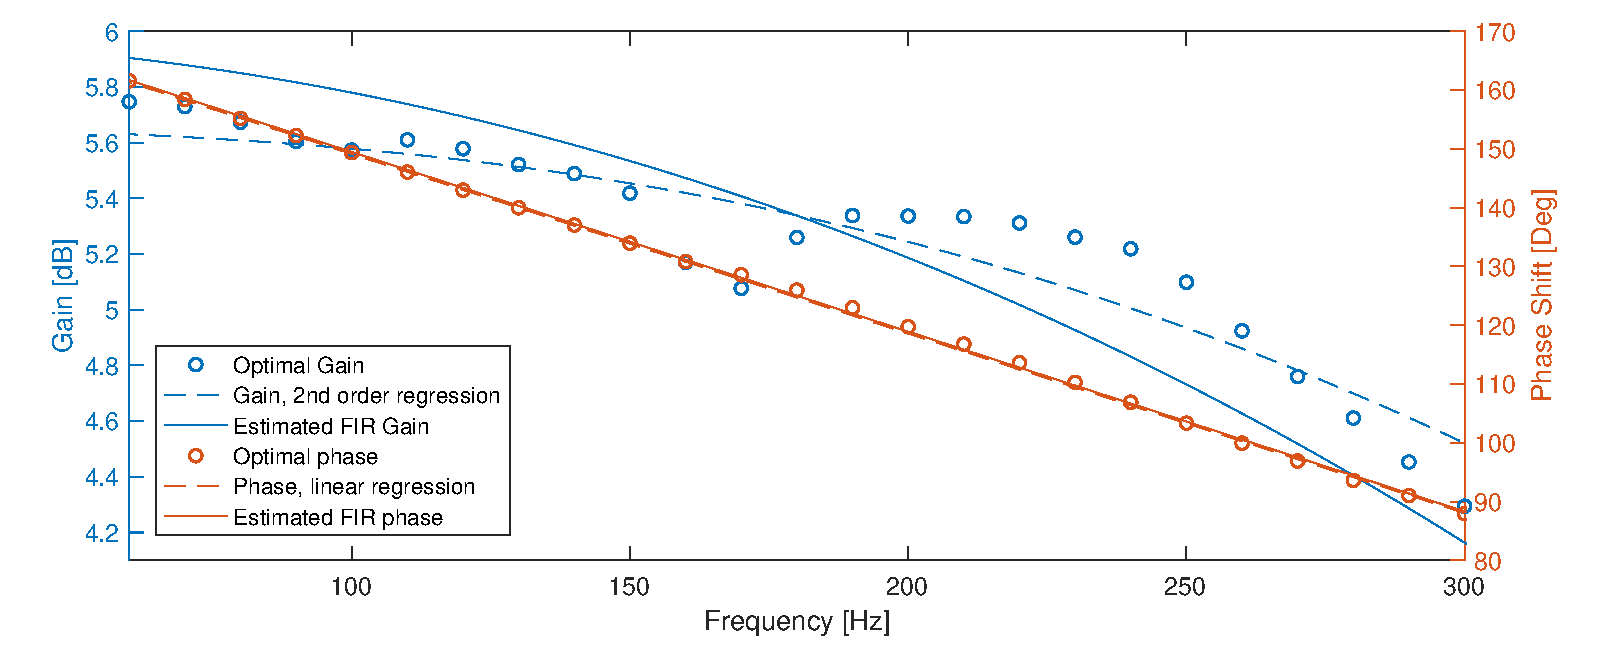
\includegraphics[width=1\textwidth]{ir_estimate_scaled_close.eps}
	\caption{The graph shows transfer function of the estimated impulse respond. The dashed line is transfer function that is needed for beam forming filter, where the blue line is the gain and the red line is the phase. The Solid line line is the transfer function of the estimated impulse response, where the blue line is the gain and the red line is the phase. All circle is the actual optimized point.}
		\label{fig:ir_estimate_scaled_close}
\end{figure}

As it can be seen at \autoref{fig:ir_estimate_scaled} that the cut off is lowered and the gain is automatic raised to the wanted area. A closer look on the area of the frequency of interest in 

It can be seen at \autoref{ir_estimate_scaled_close} that the fit is close, but the gain can be optimized. Recalling from earlier, a linear phase \gls{fir} filter have to have symmetric impulse response and therefore the impulse respond where the mirrored version is not added will be used as initial guess for the genetic optimizer. To optimize the impulse response there will be used high probability for mutation and crossover. The resend to use high probability for mutation, is that the shape of the impulse response is changed a bit for every mutation, and it is the shape there needs to be change to get the optimized \gls{fir} filter coefficient. In the mutation part, the following mutation is done.

\begin{itemize}
\item One single random chosen point in the impulse response is change by moving it up and down wards.
\item One random chosen area of the impulse response is change by moving it up and down wards with a Gaussian shape, where $\mu$ and $\sigma$ is random chosen.
\item An up-sampling is done on the impulse respond with a factor of ten. After the up-sampling the value at time zero is copied and used ans the new zero point after the impulse response is shifted one sample to the right. The resend to up-sample is that the shift only is one tenth. This technique do that the cost can be minimized more than without up-sampling. The up-sampling is done with linear interpolation. This mutation ends with a down sampling with a factor of ten such that the impulse respond is at the same length as at the start.
\item There is one mutation that only multiply a factor to the impulse respond. 
\end{itemize}

At the end of all mutation the last point of the impulse response is used as the \gls{dc} offset and the offset will be subtracted from the impulse response , such that the impulse response end at an amplitude of zero. 

\section{Result}


 

\begin{figure}[H]
	\centering
	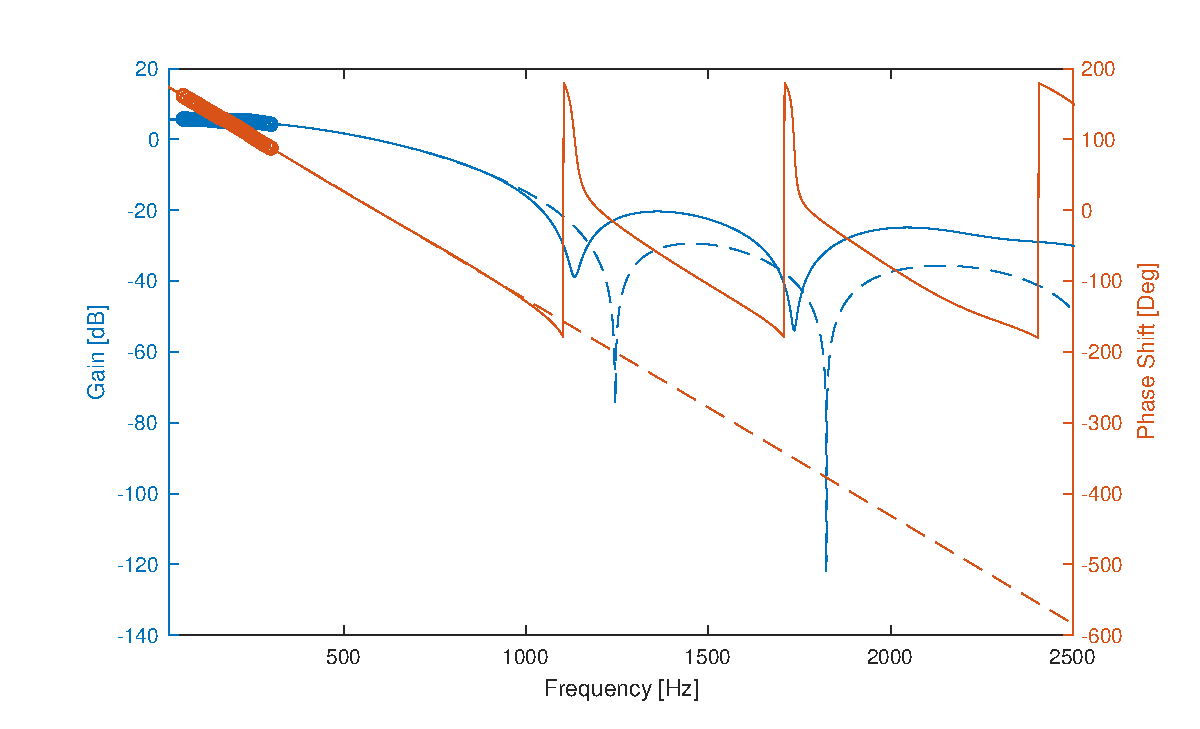
\includegraphics[width=1\textwidth]{filter_vs_reg.eps}
	\caption{The graph shows transfer function of the estimated impulse respond. The dashed line is transfer function that is needed for beam forming filter, where the blue line is the gain and the red line is the phase. The Solid line line is the transfer function of the estimated impulse response, where the blue line is the gain and the red line is the phase. All circle in the start of the graph is the actual optimized point.}
		\label{fig:filter_vs_reg}
\end{figure}

\begin{figure}[H]
	\centering
	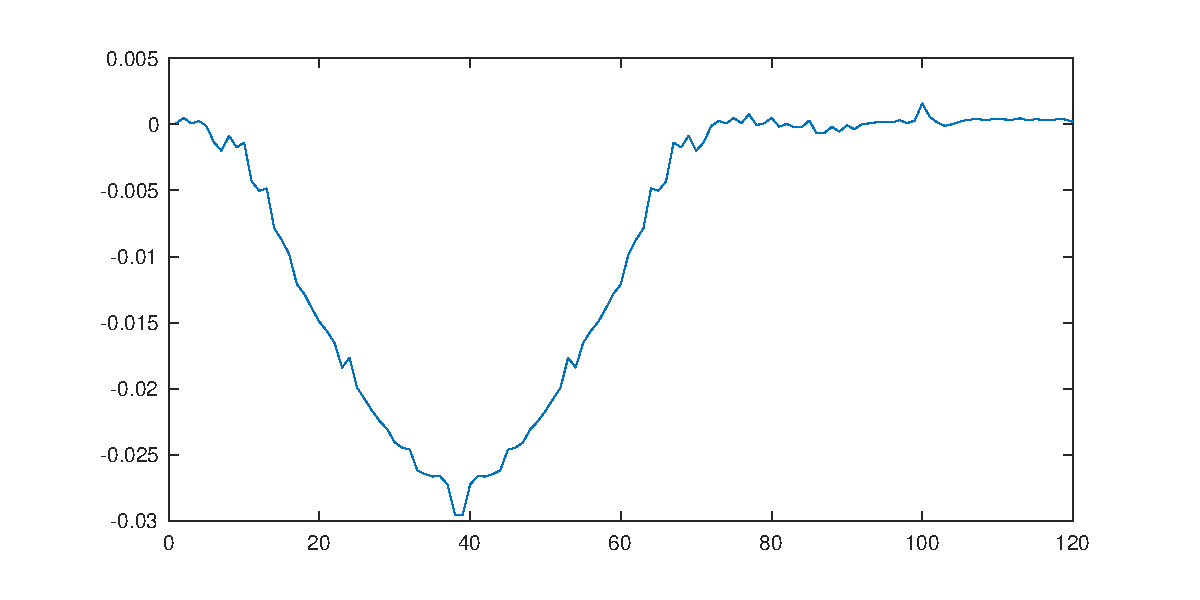
\includegraphics[width=1\textwidth]{filter_coefficient.eps}
	\caption{The graph shows the impulse respond where the mirrored version is added to the impulse respond}
		\label{fig:filter_coefficient}
\end{figure}

As it can be seen at \autoref{fig:ir_estimate_scaled} that the cut off is lowered and the gain is automatic raised to the wanted area. A closer look on the area of the frequency of interest in 


\begin{figure}[H]
\begin{subfigure}[c]{0.5\textwidth}
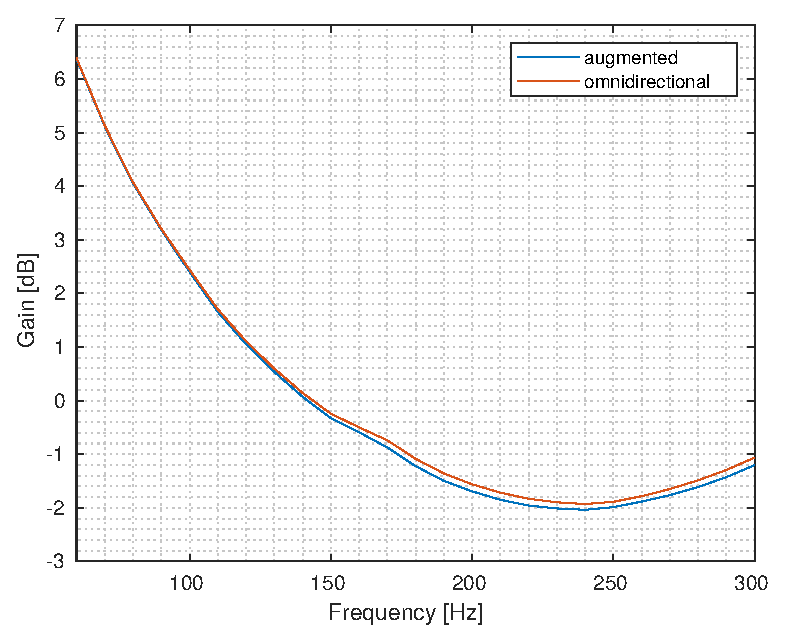
\includegraphics[width=0.85\textwidth]{opt_a.eps}
\subcaption{cost filter}
\label{fig:opt_res_a}
\end{subfigure}
\begin{subfigure}[c]{0.5\textwidth}
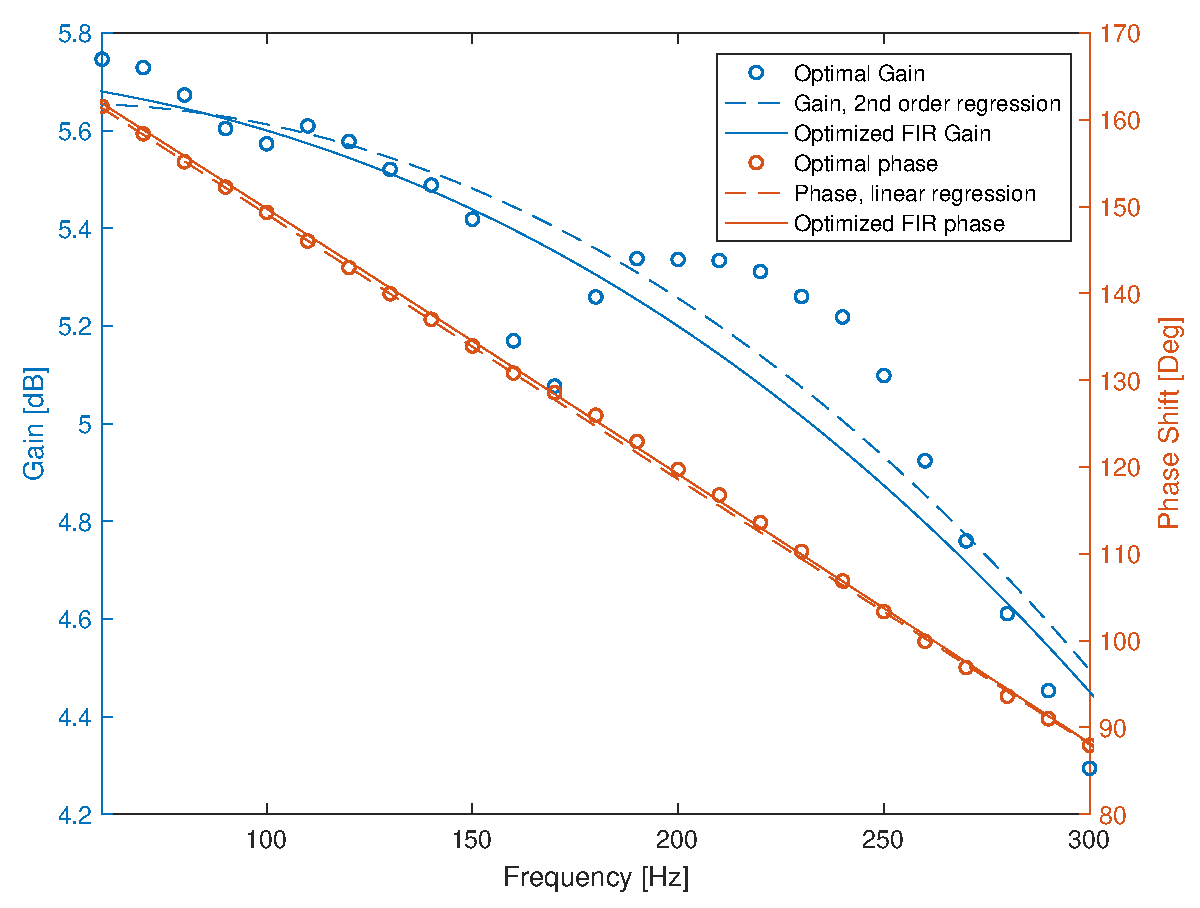
\includegraphics[width=0.95\textwidth]{filter_vs_data.eps}
\subcaption{Beamforming filter}
\label{fig:filter_vs_data}
\end{subfigure}\\
\hspace{0.1\textheight}
\begin{subfigure}[c]{0.5\textwidth}
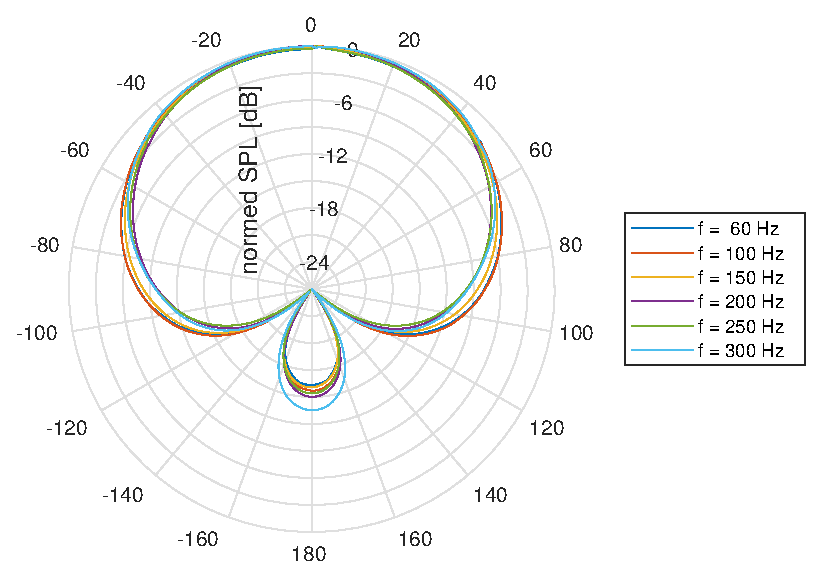
\includegraphics[width=0.95\textwidth]{opt_c.eps}
\subcaption{Directional characteristic, optimal}
\label{fig:opt_res_c}
\end{subfigure}
\begin{subfigure}[c]{0.5\textwidth}
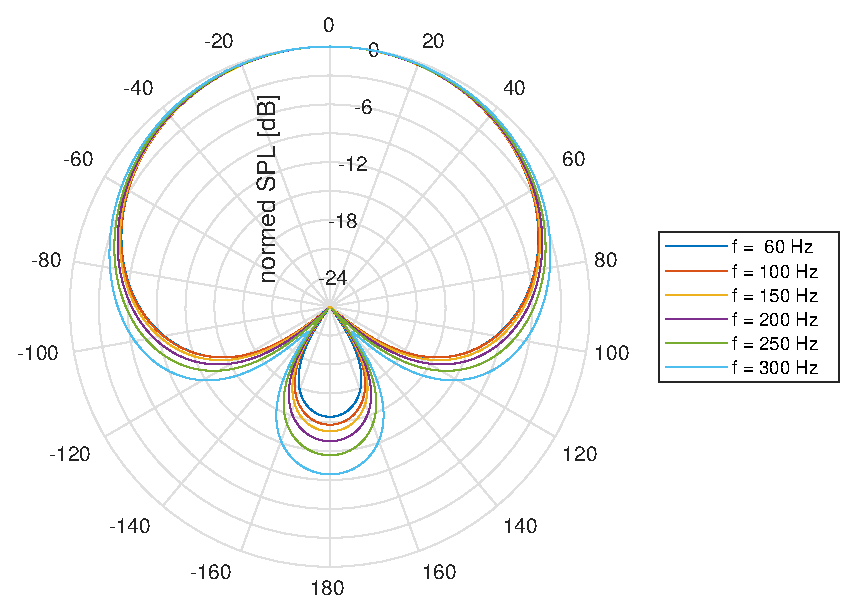
\includegraphics[width=0.95\textwidth]{polar_filtered.eps}
\subcaption{Directional characteristic, filtered}
\label{fig:polar_filtered}
\end{subfigure}
\caption{Filter results, with pressure corrected cost filter, correction table based on Appendix \ref{ax:directional_2}, \textcolor{green3}{\texttt{Lx}}\,$=$\,\SI{0.4}{\meter}, \textcolor{green3}{\texttt{Ly}}\,$=\,$\SI{-0.4}{\meter}}
		\label{fig:opt_res}
\end{figure}


\section{Conclusion}
	\chapter{Numerical Simulation}\label{ch:numerical} 
	\section{The \gls{fdtd}}
The aim of this section is to give the basic of numerical simulation by using \gls{fdtd} method, such that a speaker array sound propagation can be analysed. The method of numerical simulate one speaker will be descried, such that the method can be adapted to more than one speaker in a coupled sound pressure field. 
The theory behind \gls{fdtd} is to solve the wave equation by a finite-difference approximation for both time and space derivatives. This make it possible to easily simulate the sound propagation of a speaker in low frequency, where the speaker is omnidirectional. One of the advantage of using \gls{fdtd} is that the calculation is preformed in time domain, which benefit from that the pressure and the particle velocity at a specified time step can be analyzed directly by solving to coupled equation.\citep{fdtddaga}\\


The two equation which need to be solved is coupling the first order equation of the pressure $p$ and the particle velocity $\vec{v}$. The first formula is the Euler \autoref{fdtd_euler}, which describe the relation between the gradient for the pressure $p$ and the derivative of the particle velocity $\vec{v}$ with respect to time \autoref{fdtd_euler}. 

\begin{equation}\label{fdtd_euler}
\frac{\partial \vec{v}}{\partial t} =- \frac{1}{\rho}\vec{\triangledown }p
\end{equation}

    \startexplain
    		\explain{$\rho$ is the density of the medium }{\si{\kilo\gram\per\cubic\meter}}
        \explain{$\partial t$ is an infinitesimal time step}{\si{\second}}
        \explain{$p$ is the pressure }{\si{\pascal}}
        \explain{$\vec{v}$ is the particle velocity}{\si{\meter\per\second}}
    \stopexplain

The \autoref{fdtd_euler} is only valid with small variation of pressure. The second \autoref{fdtd_linear} is the linear continuity equation. The equation describe the relation between derivative of pressure with respect of time and the velocity gradient. They are combined by the density of the medium and the speed of sound. 

 \begin{equation}\label{fdtd_linear}
\frac{\partial p}{\partial t} =- \rho c^2 \vec{\triangledown }\vec{v}
\end{equation}

    \startexplain
    		\explain{$\rho$ is the density of the medium }{\si{\kilo\gram\per\cubic\meter}}
        \explain{$\partial t$ is an infinitesimal time step}{\si{\second}}
        \explain{$p$ is the pressure }{\si{\pascal}}
        \explain{$c$ is the speed of sound }{\si{\meter\per\second}}
        \explain{$\vec{v}$ is the particle velocity}{\si{\meter\per\second}}
    \stopexplain

Both equation are approximated using finite difference for every point in space and in time using a 3 dimensional grid of the space. 


\subsection{\gls{fdtd} using Cartesian grid}

The Cartesian grid for \gls{fdtd} approximation is a well known technique, and will be used in this project \citep{finiteproblems}. The Cartesian grid are using the pressure \autoref{fdtd_linear} and the particle velocity \autoref{fdtd_linear} as the unknown quantities, which have to be solved for every point in space. Every point in space is made out of a grid where the pressure is determined. A small grid is visualized in \autoref{fig:fdtd_cartesian_grid}

\begin{figure}[H]
	\centering
\begin{picture}(0,0)%
\includegraphics{fdtd_grid.pdf}%
\end{picture}%
\setlength{\unitlength}{4144sp}%
%
\begingroup\makeatletter\ifx\SetFigFont\undefined%
\gdef\SetFigFont#1#2#3#4#5{%
  \reset@font\fontsize{#1}{#2pt}%
  \fontfamily{#3}\fontseries{#4}\fontshape{#5}%
  \selectfont}%
\fi\endgroup%
\begin{picture}(3869,3327)(3541,-1288)
\put(6841,1649){$\delta y$}%
\put(3556,1244){z}%
\put(4006,704){x}%
\put(3826,344){y}%
\put(5806,1874){$\delta x$}%
\put(4996,-61){Pressure point}%
\put(4996,-421){Particle velocity x-direction}%
\put(4996,-781){Particle velocity y-direction}%
\put(4996,-1096){Particle velocity z-direction}%
\put(7066,704){$\delta z$}%
\end{picture}%
	\caption{A 3 dimensional example of Cartesian grid}
		\label{fig:fdtd_cartesian_grid}
\end{figure}


The grid points is build up on positions there is descried as $(i\,\delta x,j\,\delta y,k\,\delta z)$ at time $t=l$, where $\delta x,\delta y,\delta z$ is the spatial discretization step \autoref{fig:fdtd_cartesian_grid} and $\delta t$ is the time spatial discretization step. $i,j,k$ is the discrete indices for the point in grid and $l\delta t$ is the discrete time index. For every axis, the component of the particle velocity have to be determined at position in \autoref{fdtd_component} at time $t=(l+\frac{1}{2})\delta t$.

\begin{equation}\label{fdtd_component}
\vec{v}= \begin{bmatrix}
v_x[(i\pm \frac{1}{2})\,\delta x,j\,\delta y,k\,\delta z]\\
v_y[i\,\delta x,(j\pm \frac{1}{2})\,\delta y,k\,\delta z]\\
v_z[i\,\delta x,j\,\delta y,(k\pm \frac{1}{2})\,\delta z]
\end{bmatrix}
\end{equation}

The following step is done to get the linearized equation for pressure and particle velocity in Cartesian grid and with air as medium. First \autoref{fdtd_euler} has to be rewritten to \autoref{fdtd_euler_rewrite_2}


\begin{subequations}\label{fdtd_euler_rewrite}
\begin{alignat}{2}
-\rho_0 \frac{\partial \vec{v}}{\partial t} &=\vec{\triangledown }p \label{fdtd_euler_rewrite_1}\\
-\rho_0 \frac{\partial \vec{v}}{\partial t} &=\frac{\partial p}{\partial x}\vec{x}+\frac{\partial p}{\partial y}\vec{y}+\frac{\partial p}{\partial z}\vec{z} \label{fdtd_euler_rewrite_2}
\end{alignat}
\end{subequations}


Second \autoref{fdtd_linear} has to be rewritten to \autoref{fdtd_linear_rewrite_2}

\begin{subequations}\label{fdtd_linear_rewrite}
\begin{alignat}{2}
- \frac{1}{\rho_0c^2} \frac{\partial p}{\partial t} &=\vec{\triangledown }v \label{fdtd_linear_rewrite_1}\\
- \frac{1}{\rho_0c^2} \frac{\partial p}{\partial t} &=\frac{\partial v_x}{\partial x}\vec{x}+\frac{\partial v_y}{\partial y}\vec{y}+\frac{\partial v_z}{\partial z}\vec{z}\label{fdtd_linear_rewrite_2}
\end{alignat}
\end{subequations}

The linearizing of \autoref{fdtd_euler_rewrite_2} is done with combining  




\autoref{fdtd_linear_rewrite_2} 



  
		\section{\gls{fdtd} simulation} \label{sec:fdtd_simulation}
The aim of this chapter is to make a simulation of the zero order gradient speaker, first order gradient speaker and the solution proposed in \autoref{sec:opt_result} using \gls{fdtd}. All simulation cross all three different method of using speaker at low frequency will be compared in both free field and inside a room. The result will be discussed with respect to directionality and efficiency. 

\section{\gls{fdtd} simulations step size}
This section will determined the the step size for both grid size and the time step size. As the time step size is depending on the grid step size, the grid step size will be determined first. Recalling \autoref{fdtd_delta_stepsize} state that all three dimention will have the same step size in this project, the calculation is as following \autoref{fdtd_distance_stepsize} 

\begin{subequations}\label{fdtd_distance_stepsize}
\begin{alignat}{2}
d &= \delta x = \delta y = \delta z= \frac{1}{10} \frac{c}{f_{max}} \label{fdtd_distance_stepsize_1}\\
d &= \frac{1}{10} \frac{\SI{343}{\meter\per\second}}{\SI{300}{\hertz}} \label{fdtd_distance_stepsize_2}\\
d &= \SI{0.11}{\meter} \label{fdtd_distance_stepsize_3}
\end{alignat}
\end{subequations}

    \startexplain
    		\explain{$d$ is the maximum grid cell size }{\si{\meter}}
        \explain{$c$ is the speed of sound at 20 degree}{\si{\meter\per\second}}
        \explain{$f_{max}$ is the maximum frequency in the simulation}{\si{\hertz}}
    \stopexplain

Since the maximum grid cell size is \SI{0.11}{\meter}, the chosen grid cell size is in this project will be \SI{0.10}{\meter}, to be sure that a simulation does not suffer from a limiting grid cell size. The time step have to be small enough such that standard walls can be included in the simulation, and since plaster wall is well used, $Z_{1}$ is possible nonzero and therefore both condition in \autoref{sec:fdtd_time_stepsize} has to be satisfied. The first condition is \autoref{fdtd_time_stepsize_boundary} stated as following \autoref{fdtd_time_stepsize_con_one}
    
 
    \begin{subequations}\label{fdtd_time_stepsize_con_one}
\begin{alignat}{2}
\delta t &\leq \sqrt{\frac{2}{3}}  \left( \frac{1}{\sqrt{\frac{1}{(\delta x)^2}+\frac{1}{(\delta x)^2}+\frac{1}{(\delta x)^2} }\cdot c} \right)\\
\delta t &\leq \sqrt{\frac{2}{3}}  \left( \frac{1}{\sqrt{\frac{1}{(\SI{0.10}{\meter})^2}+\frac{1}{(\SI{0.10}{\meter})^2}+\frac{1}{(\SI{0.10}{\meter})^2} }\cdot \SI{343}{\meter\per\second}} \right)\\
\delta t &\leq \SI{0.137}{\milli\second} 
\end{alignat}
\end{subequations}
    
 Which correspond to a sampling frequency of at least \SI{7299}{\hertz}. The second condition is \autoref{fdtd_time_stepsize_boundary_Z_n1} where plaster is chosen as the limit case for soft walls and concrete is chosen as the limit for hard walls. The calculation for plaster walls is as following \autoref{fdtd_time_stepsize_con_plaster} \citep{finiteproblems}.
 
     \begin{subequations}\label{fdtd_time_stepsize_con_plaster}
\begin{alignat}{2}
c \delta t &\leq \delta x \left(   \frac{1+\frac{2Z_1}{\rho_0 \delta x}}{1+\frac{2Z_{-1} \delta x}{\rho_0 c^2}}  \right)^{\frac{1}{2}}\\
 \delta t &\leq \frac{\SI{0.10}{\meter} \left(   \frac{1+\frac{2\cdot 6}{1.21 \cdot \SI{0.10}{\meter}}}{1+\frac{2 \cdot 16 \cdot \SI{0.10}{\meter}}{1.21 \cdot {343}^2}}  \right)^{\frac{1}{2}}}{343}\\
\delta t &\leq \SI{2.92}{\milli\second} 
\end{alignat}
\end{subequations}
 Which correspond to a sampling frequency of at least \SI{343}{\hertz}.


concrete is missing??


It can be concluded that the grid step size $d$ shall be \SI{100}{\milli\meter} and the sampling frequency $\frac{1}{\delta t}$ shall at least be equal or higher than \SI{7399}{\hertz}, The impulse response from the used \gls{dut} will be used as the impulse response in all simulation. All impulse response measurement in this project have a sample frequency of \SI{44.1}{\kilo\hertz} but because the simulation does not have to have higher sample frequency than \SI{7399}{\hertz}, the sample frequency of the measurement will be down sampled with a factor of 6. The choose of a factor of 6 is justified by that this is the highest scalar factor the measurement sampling frequency can be down sampled  and still satisfy the minimum sampling frequency and also keeping the required process power down. This result in a sampling frequency for the simulation of \SI{7.35}{\kilo\hertz}

\section{\gls{fdtd} algorithm}
The aim of this section is to convert the grid to matrices. Since the grid is in three dimension, the whole matrix system for pressure and all particle velocity matrices will built on three dimensional matrices. The following \autoref{fig:fdtd_cartesian_grid} shows a simple grid in a corner with entry notation of $l$ as the hight of the room, $r$ as the width of the room and $c$ as the length of the room.


\begin{figure}[H]
	\centering
\begin{picture}(0,0)%
\includegraphics{fdtd_grid_matrices.pdf}%
\end{picture}%
\setlength{\unitlength}{4144sp}%
%
\begingroup\makeatletter\ifx\SetFigFont\undefined%
\gdef\SetFigFont#1#2#3#4#5{%
  \reset@font\fontsize{#1}{#2pt}%
  \fontfamily{#3}\fontseries{#4}\fontshape{#5}%
  \selectfont}%
\fi\endgroup%
\begin{picture}(3869,4070)(3541,-1873)
\put(5941,1334){\color[rgb]{0,0,1}$v_x(2,1,1)$}%
\put(4186,434){\color[rgb]{0,0,0}(r,c,l)}%
\put(5041,1019){\color[rgb]{0,0,1}$v_x(1,1,1)$}%
\put(6211,974){\color[rgb]{0,.82,0}$v_y(1,2,1)$}%
\put(5941,1604){\color[rgb]{.82,0,0}$v_z(1,1,1)$}%
\put(5041,749){\color[rgb]{.82,0,0}$v_z(1,1,2)$}%
\put(4771,1379){\color[rgb]{0,.82,0}$v_y(1,1,1)$}%
\put(5491, 74){\color[rgb]{1,0,0}$p(1,1,2)$}%
\put(6931,1199){\color[rgb]{1,0,0}$p(2,1,1)$}%
\put(6391,569){\color[rgb]{1,0,0}$p(1,2,1)$}%
\put(4996,-376){Pressure point}%
\put(4996,-736){Unknown pressure point}%
\put(3556,1244){l}%
\put(4996,-1096){Particle velocity x-direction}%
\put(4996,-1456){Particle velocity y-direction}%
\put(4006,704){r}%
\put(3826,344){c}%
\put(4996,-1771){Particle velocity z-direction}%
\end{picture}%
	\caption{The figure visualized a boundary plan through particle velocity plan $x$ in 1 dimension}
		\label{fig:fdtd_cartesian_grid}
\end{figure}





 

%%

\part{Test and Discussion}\label{pt:test}
\graphicspath{{figures/tests/}}
	\chapter{Performance Evaluation}
		%\input{chapters/tests/test_intro}
	\chapter{Comparison: Simulations and Measurement}
	\chapter{Comparison: Array vs Single Speaker}


 
%%
\part{Conclusion}\label{pt:conclusion}
%\chapter{Discussion}
\section{Comparison to a Commercial Product}
In order to get an idea of what directional characteristics have been achieved by others, the beamforming array is compared to a line array unit by the company D\&B, who specifically use their directivity control for marketing. The so called GLS8 unit is depicted in \autoref{fig:gls8_pic}. For the frequency range of this project, the key data is, that in the line array unit, two 14$^{\prime \prime}$ drivers in the front of the unit are placed, and another two 10$^{\prime \prime}$ drivers are mounted in the sides \citep{SL_GSL}[p. 6]. 
\begin{figure}[H]
\centering
\includegraphics[width=0.4\textwidth]{sl8.png}
\caption{Drawing of D\&B GLS8 line array unit, image source: \citep{SL_GSL}[p. 6]}
\label{fig:gls8_pic}
\end{figure}
The directional characteristics of the GSL8 units are depicted in \autoref{fig:gls_iso}. 
It has to be noted that this plot covers a significantly wider frequency range, than the one featured in this project. Between \SI{200}{\hertz} and \SI{300}{\hertz}, the line array unit clearly has a smaller \SI{-6}{\decibel} lobe width (approx. \SI{80}{\degree}) than the triangular array (approx. \SI{140}{\degree}), which is featured in \autoref{fig:array_iso}.
\autoref{fig:gls_iso} shows, that the lobe width for the line array module has a tendency to grow with decreasing frequency. At \SI{63}{\hertz} the \SI{-6}{\decibel} lobe width of the GSL8 unit is approx. \SI{144}{\degree}, which is in the same order of magnitude as the approx. \SI{150}{\degree} lobe width of the triangular array. When looking at these plots it has to be taken into account, that the two constructions were designed to fulfill different requirements and have very different cabinet configurations. It might be speculated, that perhaps the relatively large single cabinet of the line array unit aids directionality at higher frequencies, where at the lower end of the frequency band more of the directionality control has to be achieved by beamforming. This would explain, why at higher frequencies the lobe width of the GSL8 is clearly superior to the triangular array, while they both have similar characteristics around \SI{60}{\hertz}.
\begin{figure}[H]
\centering
	\begin{subfigure}[H]{0.7\textwidth}
		\centering
		\includegraphics[width=0.95\textwidth]{gls_isobar.png}
		\subcaption{Isobar plot for the GSL8 module, showing \SI{-6}{\decibel} and \SI{-12}{\decibel} isobars, image source: \citep{SL_GSL}[p. 9]}	
		\label{fig:gls_iso}
	\end{subfigure}\\
	\begin{subfigure}[H]{0.95\textwidth}
		\centering
		\includegraphics[width=0.95\textwidth]{dbcompare.eps}
		\subcaption{Contour plot of the relative level over frequency and angle for the triangular speaker array. Modified version of \autoref{fig:beamdwidth_array_on}, with resolution adjusted for comparison}
		\label{fig:array_iso}
	\end{subfigure}
\caption{Directional characteristics, GSL8 and triangular speaker array.}
\label{fig:isobars}
\end{figure}
\section{Applications}\label{sec:applications}
\subsection{Home application}
The beamforming array might be quite big for home application, but it may be possible to reduce the size of the beamforming array with smaller speaker units. At this point there are several possibility for home application. Imagen that the house is designed and built as an open living environment, where the kitchen and the living room is a combined open area. There might be a television with stereo speakers in the living room where the back for the television and the back of speaker points towards the kitchen. The low frequency might be an issue backwards because a low frequency driver radiate omnidirectional. At higher frequency the power is more radiated agents the person that watch television, because the high frequency driver is cardioid in it self, only the reflection reflect back to the kitchen. Because of this directionality, there might be higher pressure in the kitchen of the low frequency than the high frequency. Therefore the sound might be annoying in the kitchen because it is dominated by the low frequency. A simulation of a indoor situation with 2 speaker array is a living room is done in \autoref{fig:Indoor_simulation_60_100} and \autoref{fig:Indoor_simulation_200_300}
 




\subsection{Monitoring}
Using a normal loudspeaker as a stage monitor might lead to some complications, where the monitor and the microphone create a feedback loop or the performer is ignored by the neighbour performer monitor. The beamforming array cannot solve the feedback loop, but the beamforming array will lower the pressure in side of the monitor at low frequency and might have an useful effect. This application both have a posential at stage inside and outside. The problem of using this inside can be that the reflection is so strong that the effect do not work as intended. Another problem with monitor might be that the stage is small and there is barely space for the monitor. By adding additional input and filter for different direction of the beamforming array, it might be possible to take away three monitors and replace them by one beamforming array on such small stage. By narrow the front beam and allow higher beam at the back the sound might be possible to point on the performer as wanted. This kind of bemforming require further investigation and designing which not is done in this project. A simulation is made of a indoor application where two monitors of the beemforming array are placed on a stage, see \autoref{sec:dis:simulation}



\subsection{Main application}
The main application of the beamforming array was intended to outdoor venue, where the neighbour was the non voluntary listener. In this application where the speaker is under free field condition, it have been shown that the sound pressure can be attenuated at least \SI{-9}{\decibel} at the back and side of the array. Therefore the beamforming array will help damping the this kind of side effect of outdoor concert.


\subsection{Simulation}\label{sec:dis:simulation}
The aim of this section is to shortly investigate the wave behaver of the speaker array inside with wall reflection. This project have covered the design of the beamforming array and the behaver in free field condition. The indoor application have been keep out of interest, because of the starting point of application, which have been focused on outdoor event. The last point in the introduction was questioning the indoor application of the beamforming array. At this point there is many possibility since every room is different. The room could be a big concert hall or just a small room for living. It have been chosen to simulate a concert hall because of the monitoring application and the living room for home application. For the living room, it have been chosen to use a standard listening room of size (\SI{4.15}{\meter} x \SI{7.8}{\meter}) which correspond to the \gls{aau} standard listening room. All simulation will be done in 2 dimension because of the computation time and memory requirement. It will not give the exact simulation of the room, but since the reflection coefficient of the room wall not is measured there is already many unknown parameters in this simulation. The reflection in this simulation is done where the $Z_{-1}$ and $Z_{1}$ is unknown and set to zero, because in many case the characteristic wall impedance $Z_0$ is the predominant part \citep{fdtd_imp}. $Z_0$ can be approximated with using the absorbing coefficient \citep{fdtd_imp}. The following \autoref{eq:absorb} shows the approximated characteristic wall impedance $Z_0$ calculation

\begin{equation}\label{eq:absorb}
Z_0 = \rho c \frac{1+\sqrt{1-\alpha}}{1-\sqrt{1-\alpha}}
\end{equation}

        \startexplain
        \explain{$a$ is the absorbing coefficient}{\si{1}}
    \stopexplain
    
 The simulation give an impression of the wave behaviour in the room and not valid result. The result from a simulation of a size like the listening room is shown in \autoref{fig:Indoor_simulation_60_100} and \autoref{fig:Indoor_simulation_200_300}



\begin{figure}[H]
\begin{subfigure}[c]{0.5\textwidth}
\includegraphics[width=0.95\textwidth]{60_hz_inside_beam.eps}
\subcaption{Indoor simulation of  \SI{60}{\hertz} with beamforming}
\label{fig:Indoor_simulation_60_on}
\end{subfigure}
\begin{subfigure}[c]{0.5\textwidth}
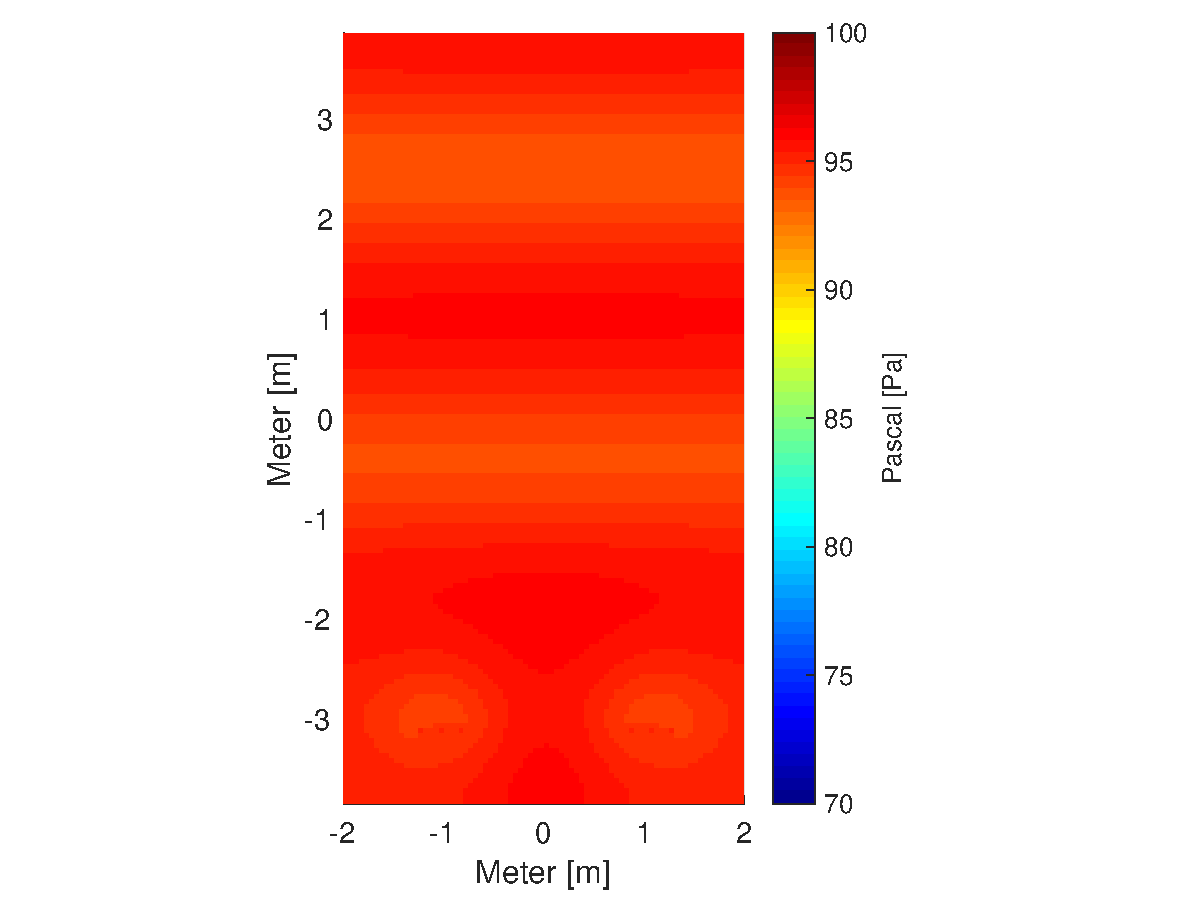
\includegraphics[width=0.95\textwidth]{60_hz_inside_without_beam.eps}
\subcaption{Indoor simulation of  \SI{60}{\hertz} without beamforming}
\label{fig:Indoor_simulation_60_off}
\end{subfigure}\\
\hspace{0.1\textheight}
\begin{subfigure}[c]{0.5\textwidth}
\includegraphics[width=0.95\textwidth]{100_hz_inside_beam.eps}
\subcaption{Indoor simulation of  \SI{100}{\hertz} with beamforming}
\label{fig:Indoor_simulation_100_on}
\end{subfigure}
\begin{subfigure}[c]{0.5\textwidth}
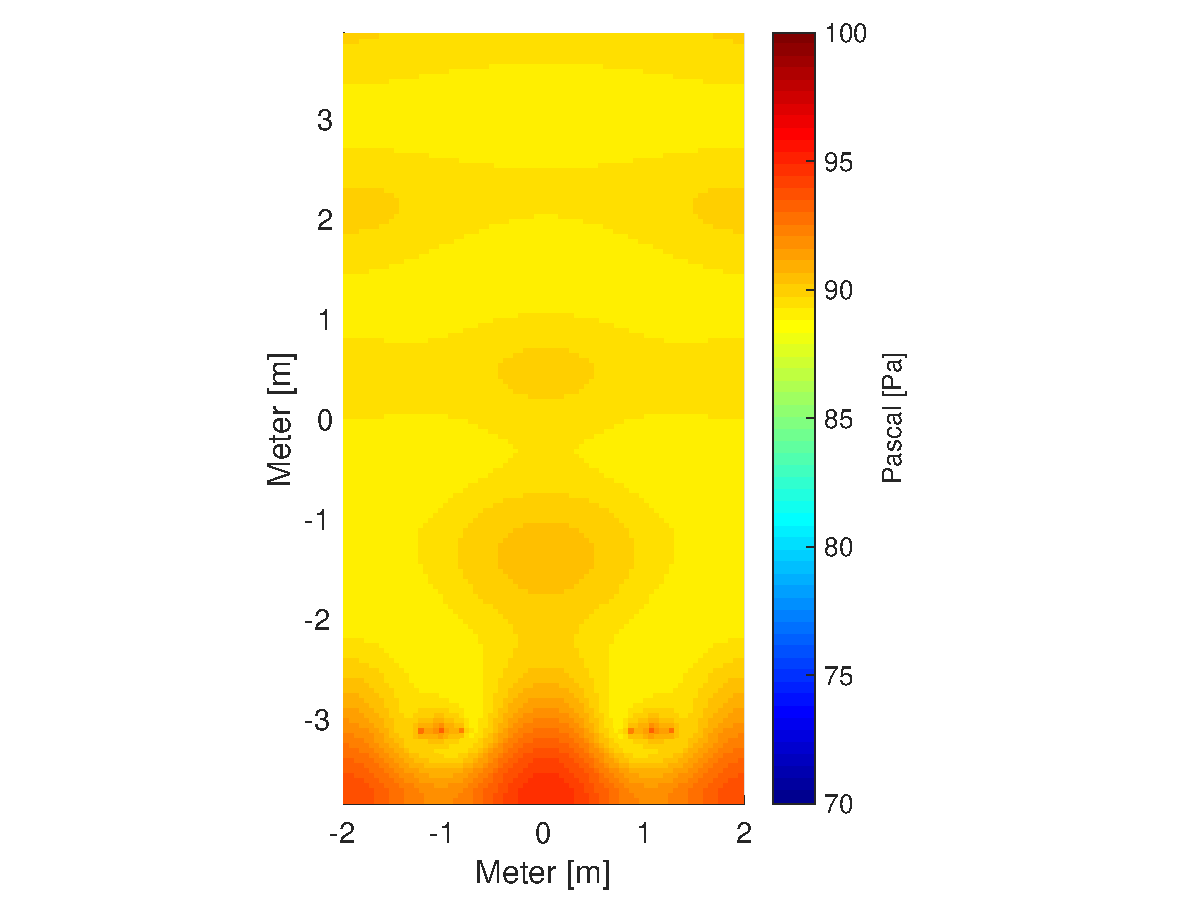
\includegraphics[width=0.95\textwidth]{100_hz_inside_without_beam.eps}
\subcaption{Indoor simulation of  \SI{100}{\hertz} with beamforming}
\label{fig:Indoor_simulation_100_off}
\end{subfigure}
\caption{The figure shows a 2 dimension \gls{fdtd} simulation in a room of size  (\SI{4.15}{\meter} x \SI{7.8}{\meter}) where the absorbing coefficient is set to 0.5}
		\label{fig:Indoor_simulation_60_100}
\end{figure}


\begin{figure}[H]
\begin{subfigure}[c]{0.5\textwidth}
\includegraphics[width=0.95\textwidth]{200_hz_inside_beam.eps}
\subcaption{Indoor simulation of  \SI{200}{\hertz} with beamforming}
\label{fig:Indoor_simulation_200_on}
\end{subfigure}
\begin{subfigure}[c]{0.5\textwidth}
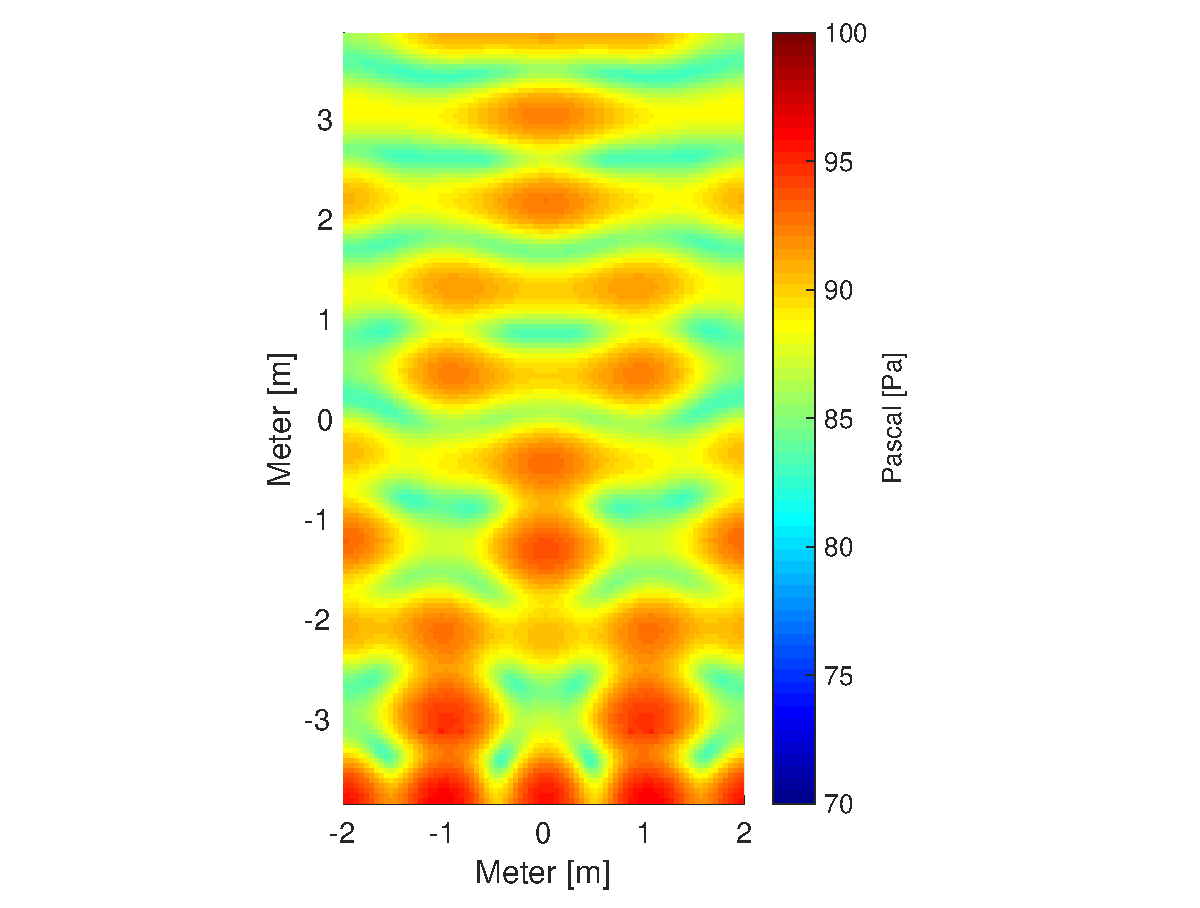
\includegraphics[width=0.95\textwidth]{200_hz_inside_without_beam.eps}
\subcaption{Indoor simulation of  \SI{200}{\hertz} without beamforming}
\label{fig:Indoor_simulation_200_off}
\end{subfigure}
\begin{subfigure}[c]{0.5\textwidth}
\includegraphics[width=0.95\textwidth]{300_hz_inside_beam.eps}
\subcaption{Indoor simulation of  \SI{300}{\hertz} with beamforming}
\label{fig:Indoor_simulation_300_on}
\end{subfigure}
\begin{subfigure}[c]{0.5\textwidth}
\includegraphics[width=0.95\textwidth]{300_hz_inside_without_beam.eps}
\subcaption{Indoor simulation of  \SI{300}{\hertz} without beamforming}
\label{fig:Indoor_simulation_300_off}
\end{subfigure}
\caption{The figure shows a 2 dimension \gls{fdtd} simulation in a room of size  (\SI{4.15}{\meter} x \SI{7.8}{\meter}) where the absorbing coefficient is set to 0.5}
		\label{fig:Indoor_simulation_200_300}
\end{figure}

In \autoref{fig:Indoor_simulation_60_100} and \autoref{fig:Indoor_simulation_200_300} it can be seen that the pressure in the room is not even ether with beamforming active or not. But one notable thing is that the pressure in the room at low frequency with omnidirectional array gets very high compare to higher frequency. So the room amplify the low frequency with reflection more that in the higher frequency area. The pressure seems to be more frequency pressure constant with beamforming active compare to beamforming disabled.\\


A second indoor application is the monitoring. In a monitoring application the room tens to be larger than a living room. The use of monitoring is often at both small and big concert where both dedicated concert hall and sports arenas are used. The following simulating example are done in a sports arena where the spectator area at sports event are on the long side of the playing field. A handball playing field do have a size of (\SI{20}{\meter}x\SI{40}{\meter}) and in this case the spectator is \SI{5}{\meter} on both long side. The following simulation \autoref{fig:Indoor_monitor_60_300} shows a simulation where the stage is placed on the top of the simulation with two monitor. Both monitors is playing upwards when looking at the simulation.


\begin{figure}[H]
\begin{subfigure}[c]{0.5\textwidth}
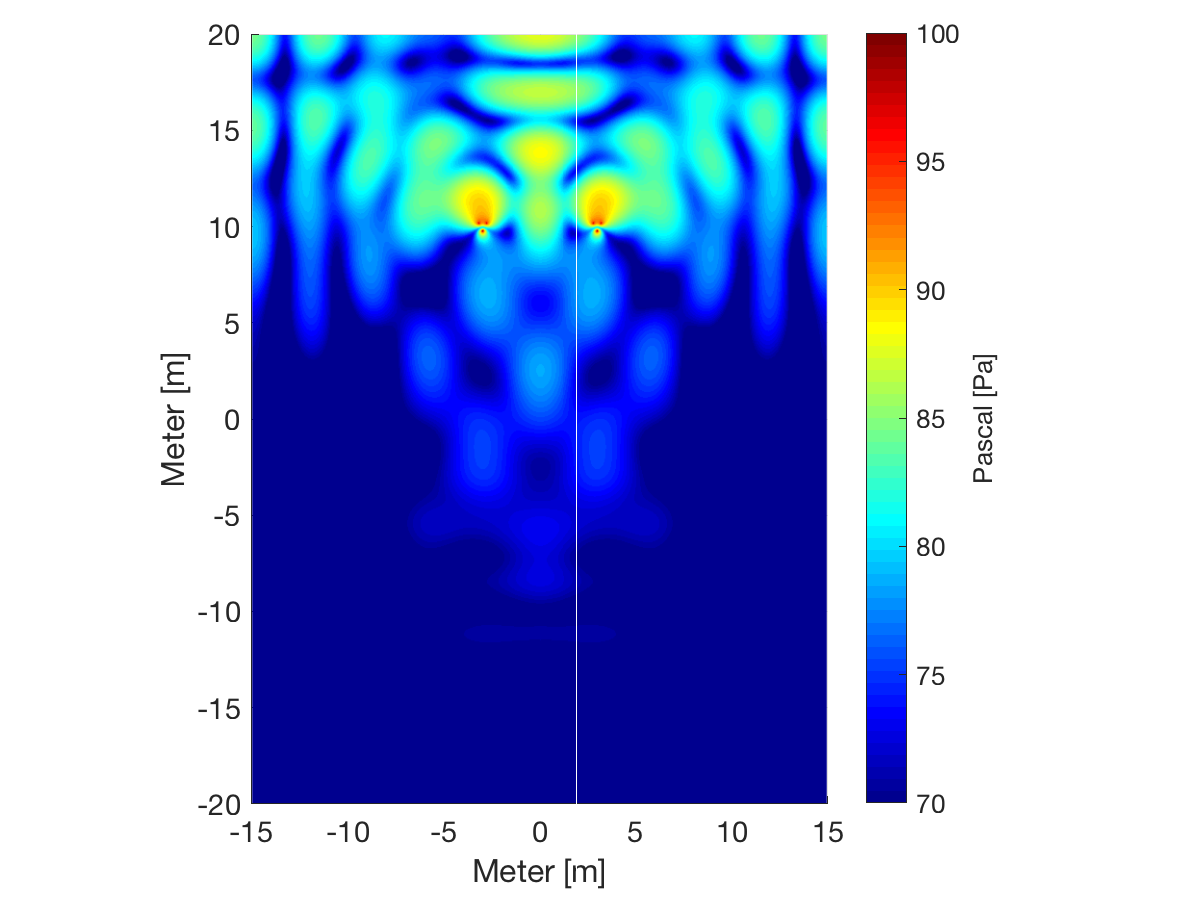
\includegraphics[width=0.95\textwidth]{60_hz_monitor_beam.eps}
\subcaption{Indoor simulation of  \SI{60}{\hertz} with beamforming}
\label{fig:Indoor_monitor_60_on}
\end{subfigure}
\begin{subfigure}[c]{0.5\textwidth}
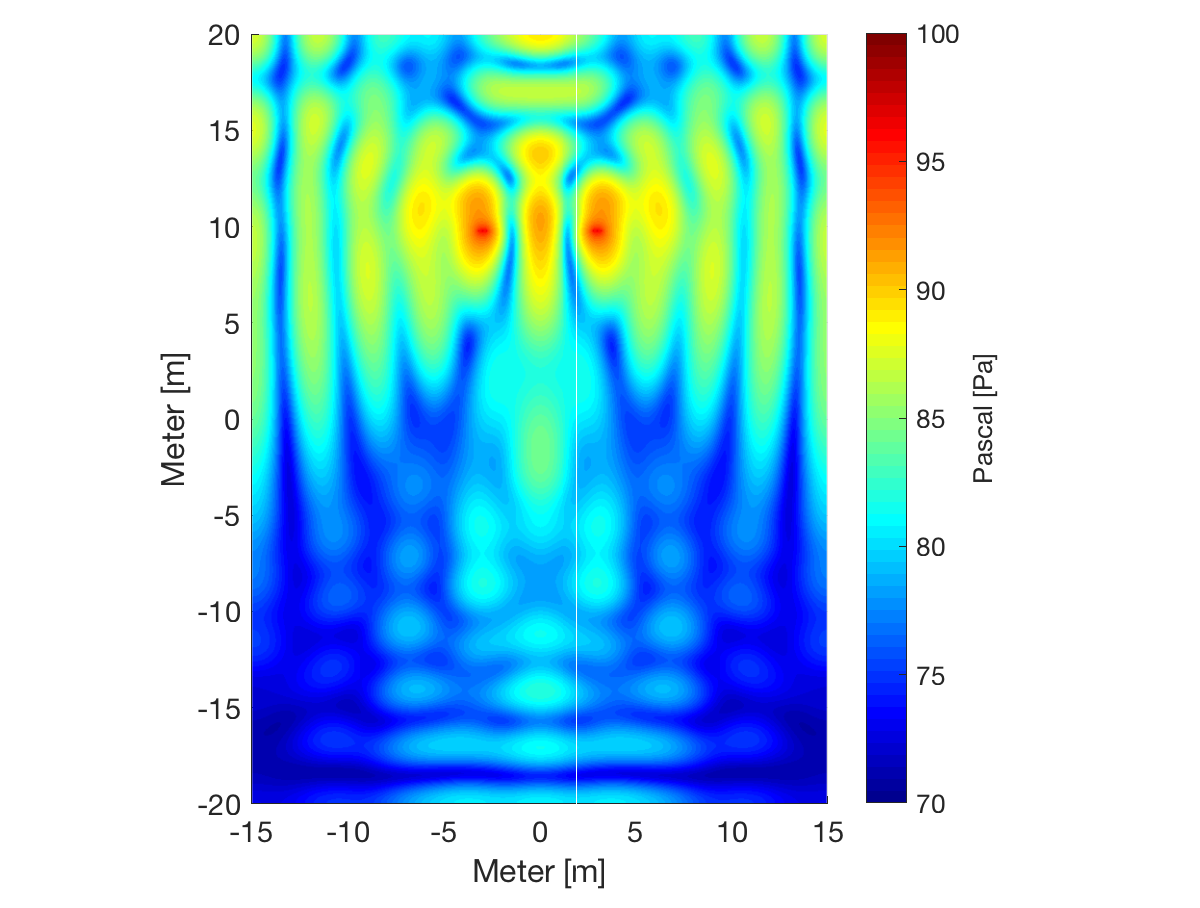
\includegraphics[width=0.95\textwidth]{60_hz_monitor_without_beam.eps}
\subcaption{Indoor simulation of  \SI{60}{\hertz} without beamforming}
\label{fig:Indoor_monitor_60_off}
\end{subfigure}\\
\hspace{0.1\textheight}
\begin{subfigure}[c]{0.5\textwidth}
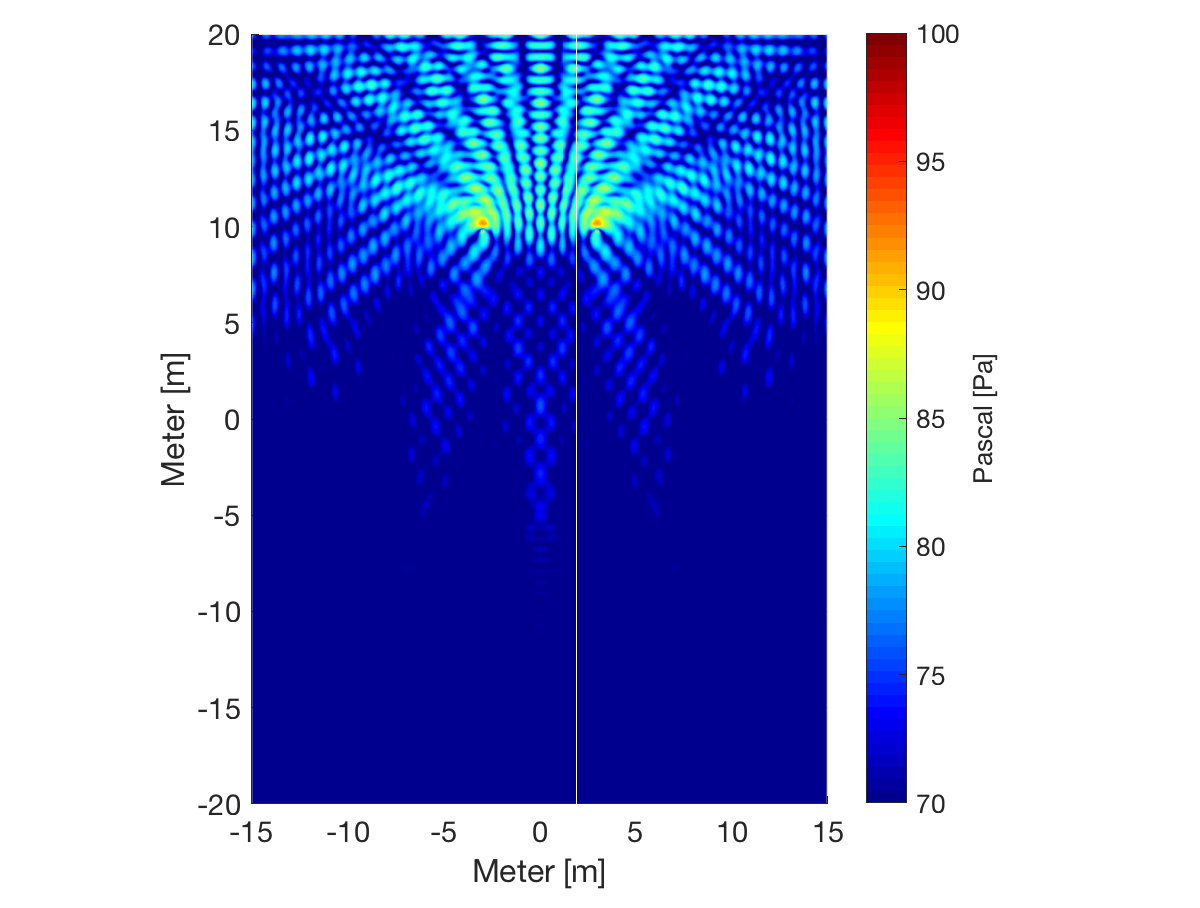
\includegraphics[width=0.95\textwidth]{300_hz_monitor_beam.eps}
\subcaption{Indoor simulation of  \SI{300}{\hertz} with beamforming}
\label{fig:Indoor_monitor_300_on}
\end{subfigure}
\begin{subfigure}[c]{0.5\textwidth}
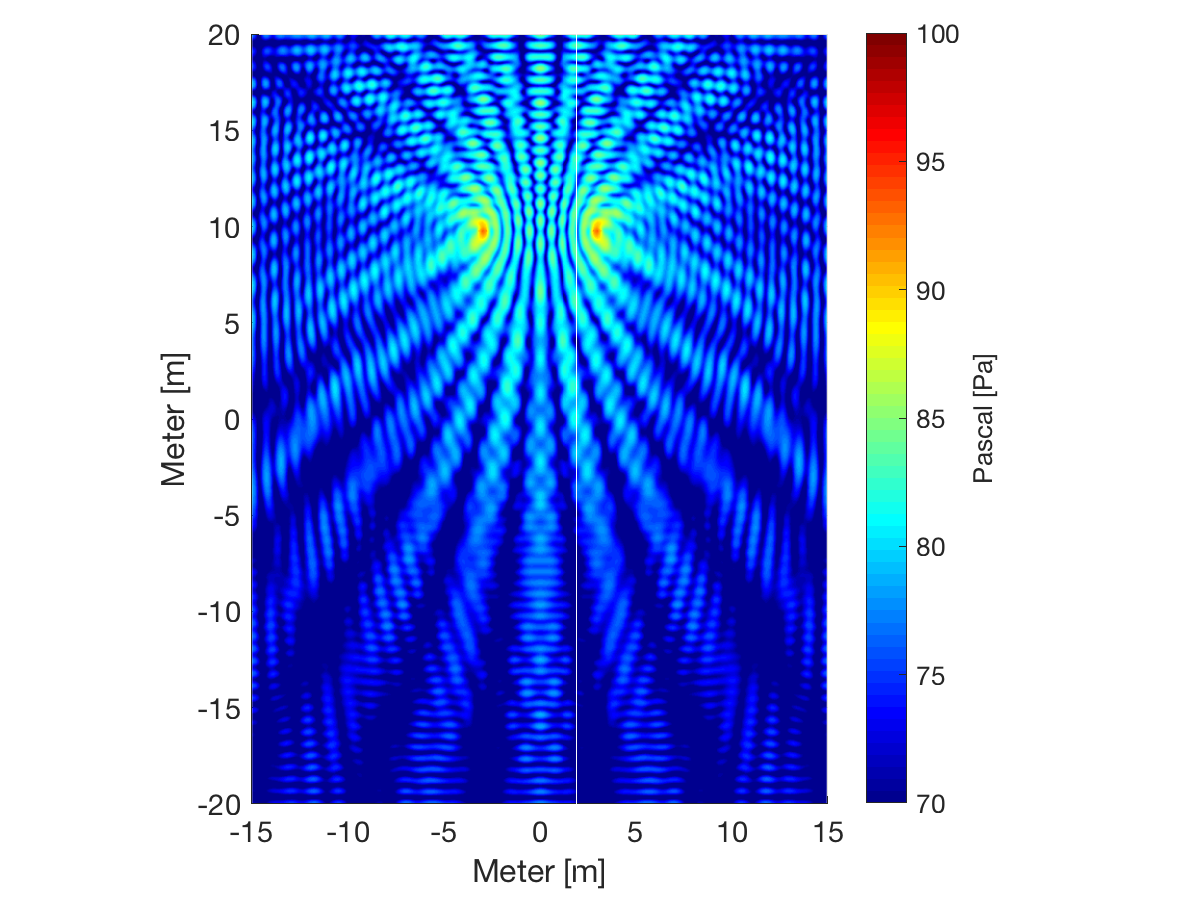
\includegraphics[width=0.95\textwidth]{300_hz_monitor_without_beam.eps}
\subcaption{Indoor simulation of  \SI{300}{\hertz} without beamforming}
\label{fig:Indoor_monitor_300_off}
\end{subfigure}
\caption{The figure shows a 2 dimension \gls{fdtd} simulation in a monitor application where the absorbing coefficient is set to 0.5}
		\label{fig:Indoor_monitor_60_300}
\end{figure}

In \autoref{fig:Indoor_monitor_60_300} it can be seen that the two monitor playing cardioid mostly have an effect on the audience and do not change much on stage. On change to the monitoring system might be that those two monitors was changed with only one beamforming monitor, but feeded with to signals and different beamforming. So one signal is playing to the left of the monitor, there the other signal was playing to the right. This concept have not been tested but it might be one possibility for change of the beamforming system.

 
%

\glsresetall
\appendix % Start of appendix
\addtocontents{toc}{\protect\setcounter{tocdepth}{0}} 
%\input{chapters/appendices/_appendices} % Include appendices
%Appendix:

 \graphicspath{{figures/appendix/}}
\part{Appendix}\label{pt:appendix}
\section{Outline ...}
In this appendix the control of the Outline turntable will be descriped    
\chapter{Measurement of Directional Characteristics I}\label{ax:directional_1}
This appendix serves as a protocol to a series of measurements conducted on the 23\textsuperscript{rd} of February 2018 in the large anechoic chamber (B4-111) at the acoustical lab of Aalborg University at Fredrik Bajers Vej 7.\\
The goal of these measurements was to try out and evaluate a MATLAB-based measurement routine to quantify the directional characteristic of loudspeakers, especially gaining experience with determining the acoustical center of a loudspeaker.

\section*{Measuring Equipment and Materials}
The following measuring equipment was used:
\begin{itemize}[noitemsep]
\item Microphone B\,\&\,K 4144
\begin{itemize}[noitemsep]
\item AAU-number: B4-109-SKF-4
\item Serial number: 297090
\end{itemize}
\item Preamplifier GRAS 26AK
\begin{itemize}[noitemsep]
\item AAU-number: B4-109-SKF-5
\item Serial number: 32811
\end{itemize}
\item Power supply B\,\&\,K 204
\begin{itemize}
\item AAU-number: B4-109-A-1
\item Serial number: 533884
\end{itemize}
\item Calibrator B\,\&\,K 4231
\begin{itemize}[noitemsep]
\item AAU-number: B4-109-A-2
\item Serial number: 2115338
\end{itemize}
\item Power Amplifier Pioneer A-616
\begin{itemize}[noitemsep]
\item AAU-number: B4-109-C-8
\item Serial number: HJ9404841S
\end{itemize}
\item Sound card RME Fireface UCX
\begin{itemize}[noitemsep]
\item AAU-number: 108230
\item Serial number: 23811948
\end{itemize}
\item Turntable: Outline ET 250-3D
\item MATLAB r2017b on OSX 10.11.6
\item Loudspeaker SEAS 33 F-WKA
\end{itemize}

The following material was used:
\begin{itemize}[noitemsep]
%\item \SI{1/2}{\inch} to \SI{1}{\inch} preamp adapter
\item Microphone clip
\item Microphone stand
\item LEMU cable
\item XLR cable
\item Ethernet cable
\item Loudspeaker stand
\item Loudspeaker cabinet, plywood, outside dimensions: (400x400x400)\SI{}{\milli\meter}, wall thickness: \SI{20}{\milli\meter}
\end{itemize}

\section*{Setup}
A sketch of the measurement setup can be found in \autoref{fig:measurement_setup}. A picture is given in \autoref{fig:setup_02_23}

\begin{figure}[htbp]
	\centering
	\includegraphics[width=0.7\textwidth]{02_23_setup.JPG}
	\caption{Measurement setup for finding the acoustical center of the speaker.}
		\label{fig:setup_02_23}
\end{figure}

The horizontal distance between the microphone and the edge of the cabinet was \SI{0.75}{\meter}. This rather short distance was deliberately chosen for the sake of determining the acoustic center of the speaker. Directivity measurements should be conducted in the far field, which in the frequency range that this project is about, loudspeaker and microphone have to be placed significantly further apart. 


\chapter{Measurement of Directional Characteristics II}\label{ax:directional_2}
This appendix serves as a protocol to a series of measurements conducted on the 2\textsuperscript{nd} of March 2018 in the large anechoic chamber (B4-111) at the acoustical lab of Aalborg University at Fredrik Bajers Vej 7.\\
The goal of these measurements was to quantify the directional characteristics of the loudspeakers that will be used in the loudspeaker array. The results are useful to show, what assumptions can be made when the speaker array is set up and where the position of the acoustic center is in relation to the cabinet. They will also serve as a baseline to which the directional characteristics of the speaker array can be compared. Furthermore, more experience can be gained regarding the practical aspects of measurement.

\section*{Measuring Equipment and Materials}
The following measuring equipment was used:
\begin{itemize}[noitemsep]
\item Microphone \gls{bandk} 4144
\begin{itemize}[noitemsep]
\item AAU-number: 06552
\item Serial number: 297090
\end{itemize}
\item Preamplifier GRAS 26AK
\begin{itemize}[noitemsep]
\item AAU-number: 56525
\item Serial number: 32811
\end{itemize}
\item Power supply \gls{bandk} 2804
\begin{itemize}
\item AAU-number: 06998
\item Serial number: 455309
\end{itemize}
\item Calibrator gls{bandk}\ 4231
\begin{itemize}[noitemsep]
\item AAU-number: 33691
\item Serial number: 2115338
\end{itemize}
\item Power Amplifier Pioneer A-616
\begin{itemize}[noitemsep]
\item AAU-number: 08249
\item Serial number: HJ9404841S
\end{itemize}
\item Sound card RME Fireface UCX
\begin{itemize}[noitemsep]
\item AAU-number: 108230
\item Serial number: 23811948
\end{itemize}
\item Turntable: Outline ET 250-3D
\begin{itemize}
\item Serial number: REIBO012
\end{itemize}
\item MATLAB r2017b on OSX 10.11.6
\item Loudspeaker SEAS 33 F-WKA
\end{itemize}

The following material was used:
\begin{itemize}[noitemsep]
%\item \SI{1/2}{\inch} to \SI{1}{\inch} preamp adapter
\item Microphone clip
\item Microphone stand
\item LEMU cable
\item XLR cable
\item Ethernet cable
\item Loudspeaker stand
\item Loudspeaker cabinet, plywood, outside dimensions: (400x400x400)\SI{}{\milli\meter}, wall~thickness:~\SI{20}{\milli\meter}
\item Speaker mount for turntable
\begin{itemize}[noitemsep]
\item Circular \gls{mdf} cutout, thickness: \SI{12}{\milli\meter}, {\(\varnothing\)~:~\SI{800}{\milli\meter}}
\item Top plate (\gls{mdf}), thickness: \SI{12}{\milli\meter}, surface : (400x400)\SI{}{\milli\meter}
\item 3 battens, (40x40x900)\SI{}{\milli\meter}
\item 3 aluminium brackets
\item 8 bolts M8x30, associated washers
\item miscellaneous woodscrews

\end{itemize}
\end{itemize}

\section*{Setup}
A sketch of the measurement setup can be found in \autoref{fig:measurement_setup}. A picture is given in \autoref{fig:setup_03_02}

\begin{figure}[htbp]
	\centering
	\includegraphics[width=0.7\textwidth]{03_02_setup.JPG}
	\caption{Measurement setup}
		\label{fig:setup_03_02}
\end{figure}

The horizontal distance between the microphone and the edge of the cabinet was \SI{2.74}{\meter}.
\chapter{Measurement of Directional Characteristics III}\label{ax:directional_3}
This appendix serves as a protocol to a series of measurements conducted between the 10\textsuperscript{th} and 12\textsuperscript{th} of May  2018 in the large anechoic chamber (B4-111) at the acoustic lab of Aalborg University at Fredrik Bajers Vej 7.\\
The goal of these measurements is investigating the behaviour of a loudspeaker array consisting of three of the loudspeakers that have been featured in \autoref{ax:directional_1} and \ref{ax:directional_2}.

\section*{Measuring Equipment and Materials}
The following measuring equipment was used:
\begin{itemize}[noitemsep]
\item Microphone \gls{bandk} 4144
\begin{itemize}[noitemsep]
\item AAU-number: 06552
\item Serial number: 297090
\end{itemize}
\item Preamplifier GRAS 26AK
\begin{itemize}[noitemsep]
\item AAU-number: 56526
\item Serial number: 32810
\end{itemize}
\item Power supply \gls{bandk} 2636
\begin{itemize}
\item AAU-number: 08022
\item Serial number: 
\end{itemize}
\item Calibrator \gls{bandk}\ 4231
\begin{itemize}[noitemsep]
\item AAU-number: 33691
\item Serial number: 2115338
\end{itemize}
\item 2 pcs. Power Amplifier Pioneer A-616
\begin{itemize}[noitemsep]
\item AAU-number: 08249, 08699
\item Serial number: HJ9404841S, JG9405804S
\end{itemize}
\item Sound card RME Fireface UCX
\begin{itemize}[noitemsep]
\item AAU-number: 108230
\item Serial number: 23811948
\end{itemize}
\item Turntable: Outline ET 250-3D
\begin{itemize}
\item Serial number: REIB0012
\end{itemize}
\item MATLAB r2017b on OSX 10.11.6
\item 3 pcs. Loudspeaker SEAS 33 F-WKA
\end{itemize}

The following material was used:
\begin{itemize}[noitemsep]
%\item \SI{1/2}{\inch} to \SI{1}{\inch} preamp adapter
\item Microphone clip
\item Microphone stand
\item LEMU cable
\item \gls{bandk} cable
\item XLR cables
\item Ethernet cable
\item miscellanious adapters
\item 3 pcs. Loudspeaker cabinet, plywood, outside dimensions: (400x400x400)\SI{}{\milli\meter}, wall~thickness:~\SI{20}{\milli\meter}, equipped with \citep{seas33}
\item Speaker mount for turntable
\begin{itemize}[noitemsep]
\item Steel mounting contraption, see REFERENCE TO HARDWARE CHAPTER
\item 3 speaker legs, \SI{40}{\milli\meter} box section, top: aluminium, {\(\varnothing\)~:~\SI{34.8}{\milli\meter}}, height: \SI{1}{\meter}
\item Circular \gls{mdf} cutout, thickness: \SI{12}{\milli\meter}, {\(\varnothing\)~:~\SI{800}{\milli\meter}}
\item \gls{mdf} cutout, thickness: \SI{20}{\milli\meter}, surface: approx. (300x600)\SI{}{\milli\meter}, bolt pattern drilled according to the bottom side of the ET 250-3D turntable
\item \gls{mdf} cutout for counterweight mounting, thickness: \SI{12}{\milli\meter}, surface : (400x400)\SI{}{\milli\meter}
\item triangular cutout (isosceles), thickness: \SI{12}{\milli\meter}, approximate outside dimensions (base width x height): (970x600)\SI{}{\milli\meter}
\item 2 Electrovoice S-200 speakers as counterweight
\item Ratchet strap
\item 4 bolts M8x80, associated washers
\item 6 bolts M8x30, associated washers
\item 8 sinkhead bolts M8x40, associated nuts and washers
\item miscellaneous woodscrews

\end{itemize}
\end{itemize}



\section*{Setup}
When setting up the speaker array according to dimensions that have been decided upon in \autoref{sec:opt_result}, a substential effort was undertaken to insure a secure stance. The turntable was mounted to one of the platform grids used in the anechoic chamber by screwing bolts through a \gls{mdf}-plate and the grid into the threads on the underside of the turntable. A round \gls{mdf} plate was mounted using the boltpattern on the upside of the turntable. Fixed to the round plate a custom made steel contraption (\autoref{fig:speakerstand}) was bolted, which itself held the legs of the speakers in place. while allowing some adjustability. In a height of approx \SI{1}{\meter} above the turntable the three speaker cabinets were mounted to the legs. On top of the speaker a triangular \gls{mdf} cutout was employed to enhance rigidity. A picture of the array is given in \autoref{fig:05_11_setup}.

\begin{figure}[h]\label{fig:05_11_setup}
	\centering
    \includegraphics[width=0.5\textwidth]{05_11_setup.jpg}
    \caption{Speaker array setup on the turntable in the anechoic chamber.}
\end{figure}

The height of the centers of the speaker cabinet above the grid turned out to be \SI{1.37}{\meter}. The microphone was set up in the same height. Platforms for the speaker array and the microphone were set up in opposing corners of the anechoic chamber, which resulted in a horizontal distance between the array center and the microphone of \SI{4.92}{\meter}.
The input and the output gain of the \gls{bandk} 2636 microphone power supply were both set to \SI{+10}{\decibel}. The input gain on the Fireface UCX was set to \SI{0}{\decibel}. On the playback side, the power amplifiers had a fixed voltage gain of \SI{+10}{\decibel} and the \texttt{playgain}-parameter in the measurement routine was set to \SI{-10}{\decibel}. The playback signals were normed so that the absolute of the biggest amplitude in on of the filtered sweeps (see \autoref{sec:filter_design} is a digital value of 1.\\
The desired positioning of the acoustic centers of the speakers was found to be describable as \texttt{Lx}$\,=\,\SI{40}{\centi\meter}$ and \texttt{Ly}$\,=\,\SI{-40}{\centi\meter}$ in \autoref{sec:opt_result}. In order to make achieve the positioning without the loudspeaker cabinets physically interfering, the azimuth of both of the two front loudspeakers \texttt{B} and \texttt{C} was rotated by \SI{50}{\degree} inwards. The speaker positions were adjusted according to the finding of \autoref{ax:directional_2}, that the acoustic center of the speaker is approx. \SI{17}{\centi\meter}. The array center was set on the rotational axis of the turntable, in order to match the way, the point sources are set up in the analytical model and the \gls{fdtd} simulation.
This positioning was used as a baseline for measurements and was later adjusted to account for imprecisions and assymetries in the way the speakers were set up and further tweaked with an heuristic approach to changing the positions in order to achieve the best possible result with the given hardware and without changing the \gls{sp}-parameters. It is assumed that these tweeks were necessary in order to account for the influence that the speaker cabinets had on the sound field. By the time of the final measurements, the rear speaker \texttt{A} had been moved towards the front by \SI{4.5}{\centi\meter}, the side speakers had been moved towards the inside by \SI{2}{\centi\meter} each, and their azimuth angle had been increased to approx. \SI{55}{\degree}.
To illustrate the way, the speakers were set up, a birdseye view is given in \autoref{fig:array_pic}.
\begin{figure}[h]\label{fig:array_pic}
	\centering
    \includegraphics[width=0.5\textwidth]{speaker_array.jpg}
    \caption{Speaker array arrangement}
\end{figure}

\section*{Results}
\chapter*{Transfer function measurement software}
In this appendix the transfer function software will be briefly explained. The gold of this software is to be able to compute the impulse response of a \gls{dut} using the logarithmic swept sine method and then compute the transfer function from the impulse response. To be able to send out a logarithmic swept sine and measure it, a full duplex soundcard have to be chosen and used as the measuring soundcard. To be able to reproduce all measurement and compare other measurement, the soundcard will not be changed doing the project work.

\section*{Materials and setup}
To measure transfer function of a \gls{dut}, the following materials are used:
\begin{itemize}
\item RME FIREFACE ucx (Soundcard)
\item MATLAB (PC - software)
\end{itemize}

\begin{figure}[htbp!]
\centering
\def\svgwidth{\columnwidth}
\chapter{Test of the Guitar's Frequency Area}\label{app:frequency_area}
A test was made to get an overview of the frequency area in which the tones from the guitar lie.

\section*{Materials and Setup}
To measure the frequency area on a guitar, the following materials are used:
\begin{itemize}
\item Digilent Analog Discovery 2 (Oscilloscope)
\item Fender Squier Classic Vibe Telecaster (Guitar)
\item Digilent Waveforms 2015 (PC - software)
\end{itemize}

\begin{figure}[htbp!]
\centering
\def\svgwidth{\columnwidth}
\chapter{Test of the Guitar's Frequency Area}\label{app:frequency_area}
A test was made to get an overview of the frequency area in which the tones from the guitar lie.

\section*{Materials and Setup}
To measure the frequency area on a guitar, the following materials are used:
\begin{itemize}
\item Digilent Analog Discovery 2 (Oscilloscope)
\item Fender Squier Classic Vibe Telecaster (Guitar)
\item Digilent Waveforms 2015 (PC - software)
\end{itemize}

\begin{figure}[htbp!]
\centering
\def\svgwidth{\columnwidth}
\input{figures/appendix/guitar_frequency_test.pdf_tex}
\caption{Setup for measuring frequency area on a guitar.}
		\label{fig:appendix:guitar_freq}
\end{figure}

\section*{Test Procedure}
To measure the frequency area on a guitar, the following steps are followed:
\begin{enumerate}
\item The materials are set up as in \autoref{fig:appendix:guitar_freq}.
\item Digilent Waveforms 2015 is set as a spectrum analyser. 
\item The guitar is set to use the neck pickup, the volume and tone control are turned all the way up to their maximum.
\item The highest and the lowest tone on the guitar are played, measured by the oscilloscope and analysed in Digilent Waveforms 2015.
\item The guitar is set to use the bridge pickup and step 4 is repeated. 
\item The data is plotted in MATLAB.
\end{enumerate}

\section*{Results}

\begin{figure}[htbp!]
	\centering
		\includegraphics[width=1\textwidth]{guitar_low_E_neck.pdf}
		\caption{Measurement of the low E note on the neck pickup.}
		\label{fig:appendix:low_E_neck}
\end{figure}

On \autoref{fig:appendix:low_E_neck} it is seen that the lowest significant frequency is around \SI{80}{\hertz} and the highest significant frequency is around \SI{500}{\hertz}, when playing the low E note on the guitar, using the neck pickup.

\newpage
\begin{figure}[htbp!]
	\centering
		\includegraphics[width=1\textwidth]{guitar_low_E_bridge.pdf}
		\caption{Measurement of the low E note on the bridge pickup.}
		\label{fig:appendix:low_E_bridge}
\end{figure}

On  \autoref{fig:appendix:low_E_bridge} it is seen that the lowest significant frequency is around \SI{80}{\hertz} and the highest significant frequency is around \SI{730}{\hertz}, when playing the low E note on the guitar, using the bridge pickup.

\begin{figure}[htbp!]
	\centering
		\includegraphics[width=1\textwidth]{guitar_high_Cis_neck.pdf}
		\caption{Measurement of the high C\# note on the neck pickup.}
		\label{fig:appendix:high_Cis_neck}
\end{figure}

On  \autoref{fig:appendix:high_Cis_neck} it is seen that the lowest significant frequency is around \SI{1100}{\hertz} and the highest significant frequency is around \SI{4400}{\hertz}, when playing the high C\# note on the guitar, using the neck pickup.

\newpage
\begin{figure}[htbp!]
	\centering
		\includegraphics[width=1\textwidth]{guitar_high_Cis_bridge.pdf}
		\caption{Measurement of the high C\# note on the bridge pickup.}
		\label{fig:appendix:high_Cis_bridge}
\end{figure}

On  \autoref{fig:appendix:high_Cis_bridge} it is seen that the lowest significant frequency is around \SI{1100}{\hertz} and the highest significant frequency is around \SI{4400}{\hertz}, when playing the high C\# note on the guitar, using the bridge pickup. 

\begin{figure}[htbp!]
	\centering
		\includegraphics[width=1\textwidth]{guitar_high_E_flasholet_bridge.pdf}
		\caption{Measurement of the high E note, played as flasholet, on the bridge pickup.}
		\label{fig:appendix:high_E_bridge_flasholet}
\end{figure}

On  \autoref{fig:appendix:high_E_bridge_flasholet} it is seen that the lowest significant frequency is around \SI{1300}{\hertz} and the highest significant frequency is around \SI{2600}{\hertz}, when playing the high E note on the guitar as flasholet, using the bridge pickup. 

\caption{Setup for measuring frequency area on a guitar.}
		\label{fig:appendix:guitar_freq}
\end{figure}

\section*{Test Procedure}
To measure the frequency area on a guitar, the following steps are followed:
\begin{enumerate}
\item The materials are set up as in \autoref{fig:appendix:guitar_freq}.
\item Digilent Waveforms 2015 is set as a spectrum analyser. 
\item The guitar is set to use the neck pickup, the volume and tone control are turned all the way up to their maximum.
\item The highest and the lowest tone on the guitar are played, measured by the oscilloscope and analysed in Digilent Waveforms 2015.
\item The guitar is set to use the bridge pickup and step 4 is repeated. 
\item The data is plotted in MATLAB.
\end{enumerate}

\section*{Results}

\begin{figure}[htbp!]
	\centering
		\includegraphics[width=1\textwidth]{guitar_low_E_neck.pdf}
		\caption{Measurement of the low E note on the neck pickup.}
		\label{fig:appendix:low_E_neck}
\end{figure}

On \autoref{fig:appendix:low_E_neck} it is seen that the lowest significant frequency is around \SI{80}{\hertz} and the highest significant frequency is around \SI{500}{\hertz}, when playing the low E note on the guitar, using the neck pickup.

\newpage
\begin{figure}[htbp!]
	\centering
		\includegraphics[width=1\textwidth]{guitar_low_E_bridge.pdf}
		\caption{Measurement of the low E note on the bridge pickup.}
		\label{fig:appendix:low_E_bridge}
\end{figure}

On  \autoref{fig:appendix:low_E_bridge} it is seen that the lowest significant frequency is around \SI{80}{\hertz} and the highest significant frequency is around \SI{730}{\hertz}, when playing the low E note on the guitar, using the bridge pickup.

\begin{figure}[htbp!]
	\centering
		\includegraphics[width=1\textwidth]{guitar_high_Cis_neck.pdf}
		\caption{Measurement of the high C\# note on the neck pickup.}
		\label{fig:appendix:high_Cis_neck}
\end{figure}

On  \autoref{fig:appendix:high_Cis_neck} it is seen that the lowest significant frequency is around \SI{1100}{\hertz} and the highest significant frequency is around \SI{4400}{\hertz}, when playing the high C\# note on the guitar, using the neck pickup.

\newpage
\begin{figure}[htbp!]
	\centering
		\includegraphics[width=1\textwidth]{guitar_high_Cis_bridge.pdf}
		\caption{Measurement of the high C\# note on the bridge pickup.}
		\label{fig:appendix:high_Cis_bridge}
\end{figure}

On  \autoref{fig:appendix:high_Cis_bridge} it is seen that the lowest significant frequency is around \SI{1100}{\hertz} and the highest significant frequency is around \SI{4400}{\hertz}, when playing the high C\# note on the guitar, using the bridge pickup. 

\begin{figure}[htbp!]
	\centering
		\includegraphics[width=1\textwidth]{guitar_high_E_flasholet_bridge.pdf}
		\caption{Measurement of the high E note, played as flasholet, on the bridge pickup.}
		\label{fig:appendix:high_E_bridge_flasholet}
\end{figure}

On  \autoref{fig:appendix:high_E_bridge_flasholet} it is seen that the lowest significant frequency is around \SI{1300}{\hertz} and the highest significant frequency is around \SI{2600}{\hertz}, when playing the high E note on the guitar as flasholet, using the bridge pickup. 

\caption{Setup for measuring frequency area on a guitar.}
		\label{fig:appendix:test}
\end{figure}

\section*{Test procedure}


\begin{enumerate}
\item The materials are set up as in \autoref{fig:appendix:test}.
\item 
\item  
\item  
\item 
\item 
\end{enumerate}

\section*{Results}

\begin{figure}[htbp!]
	\centering
		\includegraphics[width=1\textwidth]{guitar_low_E_neck.pdf}
		\caption{Measurement of the low E note on the neck pickup.}
		\label{fig:appendix:low_E_neck}
\end{figure}

On  \autoref{fig:appendix:low_E_neck} it is seen that the lowest significant frequency is around \SI{80}{\hertz} and the highest significant frequency is around \SI{400}{\hertz}, when playing the low E note on the guitar, using the neck pickup.


\chapter*{Frequency response of RME FIREFACE ucx}
A test was made to get a view of the frequency response of the RME FIREFACE ucx. The RME FIREFACE ucx is used for all measurement in this project, and therefore the frequency response is of interest. 

\section*{Materials and setup}
To measure the frequency response of the RME FIREFACE ucx, the following materials are used:
\begin{itemize}
\item RME FIREFACE ucx (Soundcard)
\item MATLAB 2017b (PC - Software)
\item jack to jack cable
\end{itemize}

\begin{figure}[htbp!]
\centering
\def\svgwidth{\columnwidth}
\chapter{Test of the Guitar's Frequency Area}\label{app:frequency_area}
A test was made to get an overview of the frequency area in which the tones from the guitar lie.

\section*{Materials and Setup}
To measure the frequency area on a guitar, the following materials are used:
\begin{itemize}
\item Digilent Analog Discovery 2 (Oscilloscope)
\item Fender Squier Classic Vibe Telecaster (Guitar)
\item Digilent Waveforms 2015 (PC - software)
\end{itemize}

\begin{figure}[htbp!]
\centering
\def\svgwidth{\columnwidth}
\chapter{Test of the Guitar's Frequency Area}\label{app:frequency_area}
A test was made to get an overview of the frequency area in which the tones from the guitar lie.

\section*{Materials and Setup}
To measure the frequency area on a guitar, the following materials are used:
\begin{itemize}
\item Digilent Analog Discovery 2 (Oscilloscope)
\item Fender Squier Classic Vibe Telecaster (Guitar)
\item Digilent Waveforms 2015 (PC - software)
\end{itemize}

\begin{figure}[htbp!]
\centering
\def\svgwidth{\columnwidth}
\input{figures/appendix/guitar_frequency_test.pdf_tex}
\caption{Setup for measuring frequency area on a guitar.}
		\label{fig:appendix:guitar_freq}
\end{figure}

\section*{Test Procedure}
To measure the frequency area on a guitar, the following steps are followed:
\begin{enumerate}
\item The materials are set up as in \autoref{fig:appendix:guitar_freq}.
\item Digilent Waveforms 2015 is set as a spectrum analyser. 
\item The guitar is set to use the neck pickup, the volume and tone control are turned all the way up to their maximum.
\item The highest and the lowest tone on the guitar are played, measured by the oscilloscope and analysed in Digilent Waveforms 2015.
\item The guitar is set to use the bridge pickup and step 4 is repeated. 
\item The data is plotted in MATLAB.
\end{enumerate}

\section*{Results}

\begin{figure}[htbp!]
	\centering
		\includegraphics[width=1\textwidth]{guitar_low_E_neck.pdf}
		\caption{Measurement of the low E note on the neck pickup.}
		\label{fig:appendix:low_E_neck}
\end{figure}

On \autoref{fig:appendix:low_E_neck} it is seen that the lowest significant frequency is around \SI{80}{\hertz} and the highest significant frequency is around \SI{500}{\hertz}, when playing the low E note on the guitar, using the neck pickup.

\newpage
\begin{figure}[htbp!]
	\centering
		\includegraphics[width=1\textwidth]{guitar_low_E_bridge.pdf}
		\caption{Measurement of the low E note on the bridge pickup.}
		\label{fig:appendix:low_E_bridge}
\end{figure}

On  \autoref{fig:appendix:low_E_bridge} it is seen that the lowest significant frequency is around \SI{80}{\hertz} and the highest significant frequency is around \SI{730}{\hertz}, when playing the low E note on the guitar, using the bridge pickup.

\begin{figure}[htbp!]
	\centering
		\includegraphics[width=1\textwidth]{guitar_high_Cis_neck.pdf}
		\caption{Measurement of the high C\# note on the neck pickup.}
		\label{fig:appendix:high_Cis_neck}
\end{figure}

On  \autoref{fig:appendix:high_Cis_neck} it is seen that the lowest significant frequency is around \SI{1100}{\hertz} and the highest significant frequency is around \SI{4400}{\hertz}, when playing the high C\# note on the guitar, using the neck pickup.

\newpage
\begin{figure}[htbp!]
	\centering
		\includegraphics[width=1\textwidth]{guitar_high_Cis_bridge.pdf}
		\caption{Measurement of the high C\# note on the bridge pickup.}
		\label{fig:appendix:high_Cis_bridge}
\end{figure}

On  \autoref{fig:appendix:high_Cis_bridge} it is seen that the lowest significant frequency is around \SI{1100}{\hertz} and the highest significant frequency is around \SI{4400}{\hertz}, when playing the high C\# note on the guitar, using the bridge pickup. 

\begin{figure}[htbp!]
	\centering
		\includegraphics[width=1\textwidth]{guitar_high_E_flasholet_bridge.pdf}
		\caption{Measurement of the high E note, played as flasholet, on the bridge pickup.}
		\label{fig:appendix:high_E_bridge_flasholet}
\end{figure}

On  \autoref{fig:appendix:high_E_bridge_flasholet} it is seen that the lowest significant frequency is around \SI{1300}{\hertz} and the highest significant frequency is around \SI{2600}{\hertz}, when playing the high E note on the guitar as flasholet, using the bridge pickup. 

\caption{Setup for measuring frequency area on a guitar.}
		\label{fig:appendix:guitar_freq}
\end{figure}

\section*{Test Procedure}
To measure the frequency area on a guitar, the following steps are followed:
\begin{enumerate}
\item The materials are set up as in \autoref{fig:appendix:guitar_freq}.
\item Digilent Waveforms 2015 is set as a spectrum analyser. 
\item The guitar is set to use the neck pickup, the volume and tone control are turned all the way up to their maximum.
\item The highest and the lowest tone on the guitar are played, measured by the oscilloscope and analysed in Digilent Waveforms 2015.
\item The guitar is set to use the bridge pickup and step 4 is repeated. 
\item The data is plotted in MATLAB.
\end{enumerate}

\section*{Results}

\begin{figure}[htbp!]
	\centering
		\includegraphics[width=1\textwidth]{guitar_low_E_neck.pdf}
		\caption{Measurement of the low E note on the neck pickup.}
		\label{fig:appendix:low_E_neck}
\end{figure}

On \autoref{fig:appendix:low_E_neck} it is seen that the lowest significant frequency is around \SI{80}{\hertz} and the highest significant frequency is around \SI{500}{\hertz}, when playing the low E note on the guitar, using the neck pickup.

\newpage
\begin{figure}[htbp!]
	\centering
		\includegraphics[width=1\textwidth]{guitar_low_E_bridge.pdf}
		\caption{Measurement of the low E note on the bridge pickup.}
		\label{fig:appendix:low_E_bridge}
\end{figure}

On  \autoref{fig:appendix:low_E_bridge} it is seen that the lowest significant frequency is around \SI{80}{\hertz} and the highest significant frequency is around \SI{730}{\hertz}, when playing the low E note on the guitar, using the bridge pickup.

\begin{figure}[htbp!]
	\centering
		\includegraphics[width=1\textwidth]{guitar_high_Cis_neck.pdf}
		\caption{Measurement of the high C\# note on the neck pickup.}
		\label{fig:appendix:high_Cis_neck}
\end{figure}

On  \autoref{fig:appendix:high_Cis_neck} it is seen that the lowest significant frequency is around \SI{1100}{\hertz} and the highest significant frequency is around \SI{4400}{\hertz}, when playing the high C\# note on the guitar, using the neck pickup.

\newpage
\begin{figure}[htbp!]
	\centering
		\includegraphics[width=1\textwidth]{guitar_high_Cis_bridge.pdf}
		\caption{Measurement of the high C\# note on the bridge pickup.}
		\label{fig:appendix:high_Cis_bridge}
\end{figure}

On  \autoref{fig:appendix:high_Cis_bridge} it is seen that the lowest significant frequency is around \SI{1100}{\hertz} and the highest significant frequency is around \SI{4400}{\hertz}, when playing the high C\# note on the guitar, using the bridge pickup. 

\begin{figure}[htbp!]
	\centering
		\includegraphics[width=1\textwidth]{guitar_high_E_flasholet_bridge.pdf}
		\caption{Measurement of the high E note, played as flasholet, on the bridge pickup.}
		\label{fig:appendix:high_E_bridge_flasholet}
\end{figure}

On  \autoref{fig:appendix:high_E_bridge_flasholet} it is seen that the lowest significant frequency is around \SI{1300}{\hertz} and the highest significant frequency is around \SI{2600}{\hertz}, when playing the high E note on the guitar as flasholet, using the bridge pickup. 

\caption{Setup for measuring frequency area on a guitar.}
		\label{fig:appendix:test}
\end{figure}

\section*{Test procedure}


\begin{enumerate}
\item The materials are set up as in \autoref{fig:appendix:test}.
\item 
\item  
\item  
\item 
\item 
\end{enumerate}

\section*{Results}

\begin{figure}[htbp!]
	\centering
		\includegraphics[width=1\textwidth]{guitar_low_E_neck.pdf}
		\caption{Measurement of the low E note on the neck pickup.}
		\label{fig:appendix:low_E_neck}
\end{figure}

On  \autoref{fig:appendix:low_E_neck} it is seen that the lowest significant frequency is around \SI{80}{\hertz} and the highest significant frequency is around \SI{400}{\hertz}, when playing the low E note on the guitar, using the neck pickup.


\chapter*{Frequency response of RME FIREFACE UCX}
A test was made to get a view of the frequency response of the Pioneer A-616 amplifier. The Pioneer A-616 amplifier is used for all measurement in this project, and therefore the frequency response is of interest. To measure the frequency response, the function from \autoref{appendix:transfer_function} is used. The test is done with and without load, to find out if the load changes the transfer function of the amplifier.

\section*{Materials and setup}
To measure the frequency response of the Pioneer A-616 amplifier, the following materials are used:
\begin{itemize}
\item RME FIREFACE UCX (Soundcard)
\item Pioneer A-616 (amplifier)
\item MATLAB 2017b (PC - Software)
\item IRmeas_fft (software) \autoref{appendix:transfer_function}
\item SEAS 33 F-WKA mounted in an enclosed 
\item XLR speaker cable
\item Jack to phone signal cable
\item Jack to banana cable
\end{itemize}

\begin{figure}[H]
\centering
\begin{picture}(0,0)%
\includegraphics{pioneer_transfer_function.pdf}%
\end{picture}%
\setlength{\unitlength}{2818sp}%
%
\begingroup\makeatletter\ifx\SetFigFont\undefined%
\gdef\SetFigFont#1#2#3#4#5{%
  \reset@font\fontsize{#1}{#2pt}%
  \fontfamily{#3}\fontseries{#4}\fontshape{#5}%
  \selectfont}%
\fi\endgroup%
\begin{picture}(8338,4926)(3838,-7474)
\put(9991,-6361){Computer}%
\put(6661,-6091){Amplifier}%
\put(9271,-3211){Sound Card}%
\put(11746,-4696){USB}%
\put(8236,-3526){Out}%
\put(8281,-3031){In}%
\put(3961,-4336){Loudspeaker}%
\put(5131,-5371){Switch}%
\end{picture}%
\caption{Setup for measuring transfer function}
		\label{fig:appendix:pioneer_response}
\end{figure}

\section*{Test procedure}


\begin{enumerate}
\item The materials are set up as in \autoref{fig:appendix:pioneer_response}.
\item The signal cable is connected between the RME FIREFACE UCX output channel 1 and right Line in on the amplifier.
\item The jack to banana cable is connected between the amplifier right B output channel to the  RME FIREFACE UCX input 1 
\item The input gain of RME FIREFACE UCX at input 1 is set to \SI{20}{\decibel}
\item The output playgain is set to \SI{-18}{\decibel}
\item The input and output channel is specified in the MATLAB function "SynchronizedPlaybackAcquirer" 
\item IRmeas_fft (software) \autoref{appendix:transfer_function} is preformed with gain \SI{-40}{\decibel}, \SI{-30}{\decibel} and \SI{-27}{\decibel} of the amplifier without load 
\item then IRmeas_fft (software) \autoref{appendix:transfer_function} is preformed with gain \SI{-40}{\decibel}, \SI{-30}{\decibel} and \SI{-27}{\decibel} of the amplifier with load 
\item To be able to measure the amplifier at higher gain, the playgain is now adjusted to \SI{-35}{\decibel}
\item  IRmeas_fft (software) \autoref{appendix:transfer_function} is preformed with gain \SI{-27}{\decibel}, \SI{-16}{\decibel} and \SI{-12}{\decibel} of the amplifier without load
\item then IRmeas_fft (software) \autoref{appendix:transfer_function} is preformed with gain \SI{-27}{\decibel}, \SI{-16}{\decibel} and \SI{-12}{\decibel} of the amplifier with load
\item The measured gain from the RME FIREFACE UCX is subtracted respectively to the playgain, to get a true voltage gain of the amplifier.
\item The transfer function is plotted from \SI{20}{\hertz} to \SI{20}{\kilo\hertz} for every measurement.

\end{enumerate}

\section*{Results}



On \autoref{fig:appendix:rme_response_result} it is seen that the soundcard only have a non linearity of \SI{0.26}{\decibel} from \SI{20}{\hertz} to \SI{20}{\kilo\hertz} between output data and input data. 

\begin{figure}[H]
	\centering
	\includegraphics[width=1\textwidth]{RME_FIREFACE_UCX_tf.pdf}
	\caption{The frequency response of the RME FIREFACE UCX with input sensitivity at 20}
		\label{fig:appendix:rme_response_result}
\end{figure}


\chapter*{Test a guitars frequency area}
In this appendix the calibration software will be briefly explained. The gold of this software is to be able to calibrate the microphone setup including the soundcard and MATLAB, scuher that a calibration tone correspond to a known digital number in MATLAB. 

\section*{Materials and setup}
To measure the .... on a guitar, the following materials are used:
\begin{itemize}
\item Digilent Analog Discovery 2 (Oscilloscope)
\item Fender Squier Classic Vibe Telecaster (Guitar)
\item Digilent Waveforms 2015 (PC - software)
\end{itemize}

%\begin{figure}[htbp!]
%\centering
%\def\svgwidth{\columnwidth}
%\chapter{Test of the Guitar's Frequency Area}\label{app:frequency_area}
A test was made to get an overview of the frequency area in which the tones from the guitar lie.

\section*{Materials and Setup}
To measure the frequency area on a guitar, the following materials are used:
\begin{itemize}
\item Digilent Analog Discovery 2 (Oscilloscope)
\item Fender Squier Classic Vibe Telecaster (Guitar)
\item Digilent Waveforms 2015 (PC - software)
\end{itemize}

\begin{figure}[htbp!]
\centering
\def\svgwidth{\columnwidth}
\chapter{Test of the Guitar's Frequency Area}\label{app:frequency_area}
A test was made to get an overview of the frequency area in which the tones from the guitar lie.

\section*{Materials and Setup}
To measure the frequency area on a guitar, the following materials are used:
\begin{itemize}
\item Digilent Analog Discovery 2 (Oscilloscope)
\item Fender Squier Classic Vibe Telecaster (Guitar)
\item Digilent Waveforms 2015 (PC - software)
\end{itemize}

\begin{figure}[htbp!]
\centering
\def\svgwidth{\columnwidth}
\input{figures/appendix/guitar_frequency_test.pdf_tex}
\caption{Setup for measuring frequency area on a guitar.}
		\label{fig:appendix:guitar_freq}
\end{figure}

\section*{Test Procedure}
To measure the frequency area on a guitar, the following steps are followed:
\begin{enumerate}
\item The materials are set up as in \autoref{fig:appendix:guitar_freq}.
\item Digilent Waveforms 2015 is set as a spectrum analyser. 
\item The guitar is set to use the neck pickup, the volume and tone control are turned all the way up to their maximum.
\item The highest and the lowest tone on the guitar are played, measured by the oscilloscope and analysed in Digilent Waveforms 2015.
\item The guitar is set to use the bridge pickup and step 4 is repeated. 
\item The data is plotted in MATLAB.
\end{enumerate}

\section*{Results}

\begin{figure}[htbp!]
	\centering
		\includegraphics[width=1\textwidth]{guitar_low_E_neck.pdf}
		\caption{Measurement of the low E note on the neck pickup.}
		\label{fig:appendix:low_E_neck}
\end{figure}

On \autoref{fig:appendix:low_E_neck} it is seen that the lowest significant frequency is around \SI{80}{\hertz} and the highest significant frequency is around \SI{500}{\hertz}, when playing the low E note on the guitar, using the neck pickup.

\newpage
\begin{figure}[htbp!]
	\centering
		\includegraphics[width=1\textwidth]{guitar_low_E_bridge.pdf}
		\caption{Measurement of the low E note on the bridge pickup.}
		\label{fig:appendix:low_E_bridge}
\end{figure}

On  \autoref{fig:appendix:low_E_bridge} it is seen that the lowest significant frequency is around \SI{80}{\hertz} and the highest significant frequency is around \SI{730}{\hertz}, when playing the low E note on the guitar, using the bridge pickup.

\begin{figure}[htbp!]
	\centering
		\includegraphics[width=1\textwidth]{guitar_high_Cis_neck.pdf}
		\caption{Measurement of the high C\# note on the neck pickup.}
		\label{fig:appendix:high_Cis_neck}
\end{figure}

On  \autoref{fig:appendix:high_Cis_neck} it is seen that the lowest significant frequency is around \SI{1100}{\hertz} and the highest significant frequency is around \SI{4400}{\hertz}, when playing the high C\# note on the guitar, using the neck pickup.

\newpage
\begin{figure}[htbp!]
	\centering
		\includegraphics[width=1\textwidth]{guitar_high_Cis_bridge.pdf}
		\caption{Measurement of the high C\# note on the bridge pickup.}
		\label{fig:appendix:high_Cis_bridge}
\end{figure}

On  \autoref{fig:appendix:high_Cis_bridge} it is seen that the lowest significant frequency is around \SI{1100}{\hertz} and the highest significant frequency is around \SI{4400}{\hertz}, when playing the high C\# note on the guitar, using the bridge pickup. 

\begin{figure}[htbp!]
	\centering
		\includegraphics[width=1\textwidth]{guitar_high_E_flasholet_bridge.pdf}
		\caption{Measurement of the high E note, played as flasholet, on the bridge pickup.}
		\label{fig:appendix:high_E_bridge_flasholet}
\end{figure}

On  \autoref{fig:appendix:high_E_bridge_flasholet} it is seen that the lowest significant frequency is around \SI{1300}{\hertz} and the highest significant frequency is around \SI{2600}{\hertz}, when playing the high E note on the guitar as flasholet, using the bridge pickup. 

\caption{Setup for measuring frequency area on a guitar.}
		\label{fig:appendix:guitar_freq}
\end{figure}

\section*{Test Procedure}
To measure the frequency area on a guitar, the following steps are followed:
\begin{enumerate}
\item The materials are set up as in \autoref{fig:appendix:guitar_freq}.
\item Digilent Waveforms 2015 is set as a spectrum analyser. 
\item The guitar is set to use the neck pickup, the volume and tone control are turned all the way up to their maximum.
\item The highest and the lowest tone on the guitar are played, measured by the oscilloscope and analysed in Digilent Waveforms 2015.
\item The guitar is set to use the bridge pickup and step 4 is repeated. 
\item The data is plotted in MATLAB.
\end{enumerate}

\section*{Results}

\begin{figure}[htbp!]
	\centering
		\includegraphics[width=1\textwidth]{guitar_low_E_neck.pdf}
		\caption{Measurement of the low E note on the neck pickup.}
		\label{fig:appendix:low_E_neck}
\end{figure}

On \autoref{fig:appendix:low_E_neck} it is seen that the lowest significant frequency is around \SI{80}{\hertz} and the highest significant frequency is around \SI{500}{\hertz}, when playing the low E note on the guitar, using the neck pickup.

\newpage
\begin{figure}[htbp!]
	\centering
		\includegraphics[width=1\textwidth]{guitar_low_E_bridge.pdf}
		\caption{Measurement of the low E note on the bridge pickup.}
		\label{fig:appendix:low_E_bridge}
\end{figure}

On  \autoref{fig:appendix:low_E_bridge} it is seen that the lowest significant frequency is around \SI{80}{\hertz} and the highest significant frequency is around \SI{730}{\hertz}, when playing the low E note on the guitar, using the bridge pickup.

\begin{figure}[htbp!]
	\centering
		\includegraphics[width=1\textwidth]{guitar_high_Cis_neck.pdf}
		\caption{Measurement of the high C\# note on the neck pickup.}
		\label{fig:appendix:high_Cis_neck}
\end{figure}

On  \autoref{fig:appendix:high_Cis_neck} it is seen that the lowest significant frequency is around \SI{1100}{\hertz} and the highest significant frequency is around \SI{4400}{\hertz}, when playing the high C\# note on the guitar, using the neck pickup.

\newpage
\begin{figure}[htbp!]
	\centering
		\includegraphics[width=1\textwidth]{guitar_high_Cis_bridge.pdf}
		\caption{Measurement of the high C\# note on the bridge pickup.}
		\label{fig:appendix:high_Cis_bridge}
\end{figure}

On  \autoref{fig:appendix:high_Cis_bridge} it is seen that the lowest significant frequency is around \SI{1100}{\hertz} and the highest significant frequency is around \SI{4400}{\hertz}, when playing the high C\# note on the guitar, using the bridge pickup. 

\begin{figure}[htbp!]
	\centering
		\includegraphics[width=1\textwidth]{guitar_high_E_flasholet_bridge.pdf}
		\caption{Measurement of the high E note, played as flasholet, on the bridge pickup.}
		\label{fig:appendix:high_E_bridge_flasholet}
\end{figure}

On  \autoref{fig:appendix:high_E_bridge_flasholet} it is seen that the lowest significant frequency is around \SI{1300}{\hertz} and the highest significant frequency is around \SI{2600}{\hertz}, when playing the high E note on the guitar as flasholet, using the bridge pickup. 

%\caption{Setup for measuring frequency area on a guitar.}
%		\label{fig:appendix:test}
%\end{figure}

\section*{Test procedure}


\begin{enumerate}
\item The materials are set up as in \autoref{fig:appendix:test}.
\item 
\item  
\item  
\item 
\item 
\end{enumerate}

\section*{Results}

%\begin{figure}[htbp!]
%	\centering
%		\includegraphics[width=1\textwidth]{guitar_low_E_neck.pdf}
%		\caption{Measurement of the low E note on the neck pickup.}
%		\label{fig:appendix:low_E_neck}
%\end{figure}

On  \autoref{fig:appendix:low_E_neck} it is seen that the lowest significant frequency is around \SI{80}{\hertz} and the highest significant frequency is around \SI{400}{\hertz}, when playing the low E note on the guitar, using the neck pickup.


\input{chapters/appendix/rme_voltage_output}
\chapter*{Speaker measuring manual}
In this appendix the \SI{360}{\degree} transfer function measurement software will be briefly explained. The gold of this software is to measure the \SI{360}{\degree} transfer function of any loudspeaker in the anicoid chamber with calibrated measuring tools. The \SI{360}{\degree} transfer function is a transfer function measurement for every specified degree step size around the speaker. E.g. if the step is one degree, the loudspeaker will be turned 1 degree for every transfer function measurement, until \SI{360}{\degree} is riched.

\section*{Materials and setup}
To measure the \SI{360}{\degree} transfer function of a loud speaker, the following materials are used:
\begin{itemize}
\item Outline ET 250-3D (Turntable)
\begin{itemize}[noitemsep]
\item AAU-number: -
\item Serial number: REIBO012
\end{itemize}
\item RME FIREFACE ucx (Soundcard)
\begin{itemize}[noitemsep]
\item AAU-number: 108230
\item Serial number: 23811948
\end{itemize}
\item Pioneer A-616 with a gain of \SI{44}{\decibel} (amplifier)
\begin{itemize}[noitemsep]
\item AAU-number: B4-109-C-8
\item Serial number: HJ9404841S
\end{itemize}
\item Microphone with preamp
\item MATLAB 2017b (PC - Software)
\item Ethernet cable 
\item \gls{bandk} connector to XLR
\item Jack to Phone cable
\item XLR speaker cable
\item speaker stand
\end{itemize}

%\begin{figure}[htbp!]
%\centering
%\def\svgwidth{\columnwidth}
%\chapter{Test of the Guitar's Frequency Area}\label{app:frequency_area}
A test was made to get an overview of the frequency area in which the tones from the guitar lie.

\section*{Materials and Setup}
To measure the frequency area on a guitar, the following materials are used:
\begin{itemize}
\item Digilent Analog Discovery 2 (Oscilloscope)
\item Fender Squier Classic Vibe Telecaster (Guitar)
\item Digilent Waveforms 2015 (PC - software)
\end{itemize}

\begin{figure}[htbp!]
\centering
\def\svgwidth{\columnwidth}
\chapter{Test of the Guitar's Frequency Area}\label{app:frequency_area}
A test was made to get an overview of the frequency area in which the tones from the guitar lie.

\section*{Materials and Setup}
To measure the frequency area on a guitar, the following materials are used:
\begin{itemize}
\item Digilent Analog Discovery 2 (Oscilloscope)
\item Fender Squier Classic Vibe Telecaster (Guitar)
\item Digilent Waveforms 2015 (PC - software)
\end{itemize}

\begin{figure}[htbp!]
\centering
\def\svgwidth{\columnwidth}
\input{figures/appendix/guitar_frequency_test.pdf_tex}
\caption{Setup for measuring frequency area on a guitar.}
		\label{fig:appendix:guitar_freq}
\end{figure}

\section*{Test Procedure}
To measure the frequency area on a guitar, the following steps are followed:
\begin{enumerate}
\item The materials are set up as in \autoref{fig:appendix:guitar_freq}.
\item Digilent Waveforms 2015 is set as a spectrum analyser. 
\item The guitar is set to use the neck pickup, the volume and tone control are turned all the way up to their maximum.
\item The highest and the lowest tone on the guitar are played, measured by the oscilloscope and analysed in Digilent Waveforms 2015.
\item The guitar is set to use the bridge pickup and step 4 is repeated. 
\item The data is plotted in MATLAB.
\end{enumerate}

\section*{Results}

\begin{figure}[htbp!]
	\centering
		\includegraphics[width=1\textwidth]{guitar_low_E_neck.pdf}
		\caption{Measurement of the low E note on the neck pickup.}
		\label{fig:appendix:low_E_neck}
\end{figure}

On \autoref{fig:appendix:low_E_neck} it is seen that the lowest significant frequency is around \SI{80}{\hertz} and the highest significant frequency is around \SI{500}{\hertz}, when playing the low E note on the guitar, using the neck pickup.

\newpage
\begin{figure}[htbp!]
	\centering
		\includegraphics[width=1\textwidth]{guitar_low_E_bridge.pdf}
		\caption{Measurement of the low E note on the bridge pickup.}
		\label{fig:appendix:low_E_bridge}
\end{figure}

On  \autoref{fig:appendix:low_E_bridge} it is seen that the lowest significant frequency is around \SI{80}{\hertz} and the highest significant frequency is around \SI{730}{\hertz}, when playing the low E note on the guitar, using the bridge pickup.

\begin{figure}[htbp!]
	\centering
		\includegraphics[width=1\textwidth]{guitar_high_Cis_neck.pdf}
		\caption{Measurement of the high C\# note on the neck pickup.}
		\label{fig:appendix:high_Cis_neck}
\end{figure}

On  \autoref{fig:appendix:high_Cis_neck} it is seen that the lowest significant frequency is around \SI{1100}{\hertz} and the highest significant frequency is around \SI{4400}{\hertz}, when playing the high C\# note on the guitar, using the neck pickup.

\newpage
\begin{figure}[htbp!]
	\centering
		\includegraphics[width=1\textwidth]{guitar_high_Cis_bridge.pdf}
		\caption{Measurement of the high C\# note on the bridge pickup.}
		\label{fig:appendix:high_Cis_bridge}
\end{figure}

On  \autoref{fig:appendix:high_Cis_bridge} it is seen that the lowest significant frequency is around \SI{1100}{\hertz} and the highest significant frequency is around \SI{4400}{\hertz}, when playing the high C\# note on the guitar, using the bridge pickup. 

\begin{figure}[htbp!]
	\centering
		\includegraphics[width=1\textwidth]{guitar_high_E_flasholet_bridge.pdf}
		\caption{Measurement of the high E note, played as flasholet, on the bridge pickup.}
		\label{fig:appendix:high_E_bridge_flasholet}
\end{figure}

On  \autoref{fig:appendix:high_E_bridge_flasholet} it is seen that the lowest significant frequency is around \SI{1300}{\hertz} and the highest significant frequency is around \SI{2600}{\hertz}, when playing the high E note on the guitar as flasholet, using the bridge pickup. 

\caption{Setup for measuring frequency area on a guitar.}
		\label{fig:appendix:guitar_freq}
\end{figure}

\section*{Test Procedure}
To measure the frequency area on a guitar, the following steps are followed:
\begin{enumerate}
\item The materials are set up as in \autoref{fig:appendix:guitar_freq}.
\item Digilent Waveforms 2015 is set as a spectrum analyser. 
\item The guitar is set to use the neck pickup, the volume and tone control are turned all the way up to their maximum.
\item The highest and the lowest tone on the guitar are played, measured by the oscilloscope and analysed in Digilent Waveforms 2015.
\item The guitar is set to use the bridge pickup and step 4 is repeated. 
\item The data is plotted in MATLAB.
\end{enumerate}

\section*{Results}

\begin{figure}[htbp!]
	\centering
		\includegraphics[width=1\textwidth]{guitar_low_E_neck.pdf}
		\caption{Measurement of the low E note on the neck pickup.}
		\label{fig:appendix:low_E_neck}
\end{figure}

On \autoref{fig:appendix:low_E_neck} it is seen that the lowest significant frequency is around \SI{80}{\hertz} and the highest significant frequency is around \SI{500}{\hertz}, when playing the low E note on the guitar, using the neck pickup.

\newpage
\begin{figure}[htbp!]
	\centering
		\includegraphics[width=1\textwidth]{guitar_low_E_bridge.pdf}
		\caption{Measurement of the low E note on the bridge pickup.}
		\label{fig:appendix:low_E_bridge}
\end{figure}

On  \autoref{fig:appendix:low_E_bridge} it is seen that the lowest significant frequency is around \SI{80}{\hertz} and the highest significant frequency is around \SI{730}{\hertz}, when playing the low E note on the guitar, using the bridge pickup.

\begin{figure}[htbp!]
	\centering
		\includegraphics[width=1\textwidth]{guitar_high_Cis_neck.pdf}
		\caption{Measurement of the high C\# note on the neck pickup.}
		\label{fig:appendix:high_Cis_neck}
\end{figure}

On  \autoref{fig:appendix:high_Cis_neck} it is seen that the lowest significant frequency is around \SI{1100}{\hertz} and the highest significant frequency is around \SI{4400}{\hertz}, when playing the high C\# note on the guitar, using the neck pickup.

\newpage
\begin{figure}[htbp!]
	\centering
		\includegraphics[width=1\textwidth]{guitar_high_Cis_bridge.pdf}
		\caption{Measurement of the high C\# note on the bridge pickup.}
		\label{fig:appendix:high_Cis_bridge}
\end{figure}

On  \autoref{fig:appendix:high_Cis_bridge} it is seen that the lowest significant frequency is around \SI{1100}{\hertz} and the highest significant frequency is around \SI{4400}{\hertz}, when playing the high C\# note on the guitar, using the bridge pickup. 

\begin{figure}[htbp!]
	\centering
		\includegraphics[width=1\textwidth]{guitar_high_E_flasholet_bridge.pdf}
		\caption{Measurement of the high E note, played as flasholet, on the bridge pickup.}
		\label{fig:appendix:high_E_bridge_flasholet}
\end{figure}

On  \autoref{fig:appendix:high_E_bridge_flasholet} it is seen that the lowest significant frequency is around \SI{1300}{\hertz} and the highest significant frequency is around \SI{2600}{\hertz}, when playing the high E note on the guitar as flasholet, using the bridge pickup. 

%\caption{Setup for measuring frequency area on a guitar.}
%		\label{fig:appendix:test}
%\end{figure}

\section*{Calibration procedure}


\begin{enumerate}
\item The materials are set up as in \autoref{appendix:calibration}.
\item NOTE! The calibration shall be done in the same order as the following description.
\item The sound card is calibrated according to the first step in \autoref{apendix:calibrate_sound_card_and_microphone}   
\item The microphone is calibrated according to the second step in \autoref{apendix:calibrate_sound_card_and_microphone}
\end{enumerate}

\section*{Test procedure}


\begin{enumerate}
\item The materials are set up as in \autoref{fig:appendix}.
\item The turn degree step is chosen and the turntable control software \autoref{appendix:turntable} is used.  
\item  All transfer function for every step is stored in complex value together with the impulse response.
\end{enumerate}


%\begin{figure}[htbp!]
%	\centering
	%	\includegraphics[width=1\textwidth]{guitar_low_E_neck.pdf}
		%\caption{Measurement of the low E note on the neck pickup.}
%		\label{fig:appendix:low_E_neck}
%\end{figure}

\section*{The MATLAB function}

\includeCode{transfer_measure.m}{matlab}{1}{55}{The \SI{360}{\degree} transfer function measurement software}{code:transfer_measure}{./code/acoustics_center_002_02_2018/}


\chapter*{Test a guitars frequency area}
In this appendix the beamwidth calculation software will be briefly explained. The gold of the software is to find the $-n$\si{\decibel} beamwidth of an arbitrary speaker, where the polar response is measured. 

\section*{Materials}
To calculate the $-n$\si{\decibel} beamwidth, the following materials are used:
\begin{itemize}
\item MATLAB 2017b (PC - software)
\end{itemize}


\section*{Test procedure}


\begin{enumerate}
\item The materials are set up as in \autoref{fig:measurement_setup}.
\item The polar response is measured according to \autoref{appendix:measuring_manual}
\item  
\item  
\item 
\item 
\end{enumerate}




\input{chapters/appendix/optimization_code}


